\documentclass[a4paper,11pt,fleqn,twoside,openright]{memoir} 	% Openright aabner kapitler paa hoejresider (openany = vilkaarlig/begge)

%%%% PAKKER %%%%

% ¤¤ Oversaettelse og tegnsaetning ¤¤ %
\usepackage[utf8]{inputenc}					% Input-indkodning af tegnsaet, dvs. input fra keyboard, tegnoversigt eller andet (UTF8 = Unicode)
\usepackage[T1]{fontenc}					% Output-indkodning af tegnsaet, dvs. printede fonte og tegn (T1 = Type 1 font med support for de fleste europaeiske sprog)
\usepackage[danish]{babel}					% Sproglig fremstilling af elementer (figur vs. figure, litteratur vs. bibliography osv.)
\usepackage{ragged2e,anyfontsize}			% Justering af elementer
																			
% ¤¤ Figurer og tabeller (floats) ¤¤ %
\usepackage{longtable}
\usepackage{graphicx} 						% Inkludering af eksterne billeder (JPG, PNG, PDF)
\usepackage{multirow}                		% Fletning af raekker og kolonner (\multicolumn og \multirow)
\usepackage{colortbl} 						% Farver i tabeller (fx \columncolor, \rowcolor og \cellcolor)
\usepackage[dvipsnames]{xcolor}				% Definer farver med \definecolor. Se mere: http://en.wikibooks.org/wiki/LaTeX/Colors
\usepackage{flafter}						% Soerger for, at floats ikke optraeder i teksten foer deres reference
\usepackage{float}							% Muliggoer eksakt placering af floats, fx \begin{figure}[H]
\let\newfloat\relax 						% Justering mellem float-pakken og memoir
%\usepackage{eso-pic}						% Tilfoej billedekommandoer paa hver side
%\usepackage{wrapfig}						% Indsaettelse af figurer omsvoebt af tekst 
%\usepackage{multicol}         	        	% Muliggoer tekst i spalter
%\usepackage{rotating}						% Rotation af tekst med \begin{sideways}...\end{sideways}

% ¤¤ Matematik mm. ¤¤
\usepackage{amsmath,amssymb,stmaryrd} 		% Avancerede matematik-udvidelser
\usepackage{mathtools}						% Andre matematik- og tegnudvidelser
\usepackage{textcomp}                 		% Symbol-udvidelser (fx promille-tegn med \textperthousand)
\usepackage{siunitx}						% Flot og konsistent praesentation af tal og enheder med \si{enhed} og \SI{tal}{enhed}
\sisetup{output-decimal-marker = {,}}		% Opsaetning af \SI og decimalseparator
%\usepackage[version=3]{mhchem} 			% Kemi-pakke til flot og let notation af formler, fx \ce{Fe2O3}
%\usepackage{rsphrase}						% Kemi-pakke til RS-saetninger, fx \rsphrase{R1}

% ¤¤ Referencer og kilder ¤¤ %
\usepackage[danish]{varioref}				% Muliggoer bl.a. krydshenvisninger med sidetal (\vref)
%\usepackage{natbib}				% Udvidelse med naturvidenskabelige citationsmodeller, herunder Harvard-modellen
%\usepackage{xr}							% Referencer til eksternt dokument med \externaldocument{<NAVN>}
%\usepackage{glossaries}					% Terminologi- eller symbolliste (se mere i Lars Madsens Latex-bog)
\usepackage[numbers]{natbib}

% ¤¤ Misc. ¤¤ %
\usepackage{listings}						% Placer kildekode i dokumentet med \begin{lstlisting}...\end{lstlisting}
\usepackage{lipsum}							% Dummy tekst med fx \lipsum[2]
\usepackage[shortlabels]{enumitem}			% Muliggoer enkelt konfiguration af lister (se \setlist nedenfor)
\usepackage{pdfpages}						% Goer det muligt at inkludere pdf-dokumenter med kommandoen \includepdf[pages={x-y}]{fil.pdf}	
\pdfoptionpdfminorversion=6					% Muliggoer inkludering af pdf-dokumenter af version 1.6 og hoejere
\pretolerance=2500 							% Justering af afstand mellem ord (hoejt tal, mindre orddeling og mere luft mellem ord)

% Kommentarer og rettelser med \fxnote. Med 'final' i stedet for 'draft' udloeser hver note en error i den faerdige rapport.
\usepackage[footnote,draft,danish,silent,nomargin]{fixme}		


%%%% BRUGERDEFINEREDE INDSTILLINGER %%%%

% ¤¤ Marginer ¤¤ %
\setlrmarginsandblock{3.5cm}{2.5cm}{*}		% \setlrmarginsandblock{Indbinding}{Kant}{Ratio}
\setulmarginsandblock{2.5cm}{3.0cm}{*}		% \setulmarginsandblock{Top}{Bund}{Ratio}
\checkandfixthelayout 						% Oversaetter vaerdier til brug for andre pakker

%	¤¤ Afsnitsformatering ¤¤ %
\setlength{\parindent}{0mm}           		% Stoerrelse af indryk
\setlength{\parskip}{3mm}          			% Afstand mellem afsnit ved brug af double Enter
\linespread{1,1}							% Linjeafstand

% ¤¤ Litteraturlisten ¤¤ %
%\bibpunct[,]{[}{]}{;}{a}{,}{,} 				% Definerer parametre ved Harvard-henvisning (bl.a. parantestype og seperatortegn)	
%\bibliographystyle{bibtex/harvard}		% Udseende af litteraturlisten (Harvard-metoden - skift til fx 'plain' for tal)
\bibliographystyle{unsrt}

% ¤¤ Dybde af overskrifter ¤¤ %
\setsecnumdepth{subsection}		 			% Dybden af nummerede overkrifter (part/chapter/section/subsection)
\setsecnumdepth{subsubsection}
\settocdepth{subsection} 					% Dybden af overskrifter vist i indholdsfortegnelsen

% ¤¤ Lister ¤¤ %
\setlist{
  topsep=0pt,								% Vertikal afstand mellem tekst og listen
  itemsep=-1ex,								% Vertikal afstand mellem items
} 

% ¤¤ Visuelle referencer ¤¤ %
\usepackage[colorlinks]{hyperref}			% Danner klikbare referencer (hyperlinks) i dokumentet
\hypersetup{colorlinks = true,				% Opsaetning af farvede hyperlinks (interne links, citeringer og URL)
    linkcolor = black,
    citecolor = black,
    urlcolor = black
}

% ¤¤ Opsaetning af figur- og tabeltekst ¤¤ %
\captionnamefont{\small\bfseries\itshape}	% Opsaetning af tekstdelen ('Figur' eller 'Tabel')
\captiontitlefont{\small}					% Opsaetning af nummerering
\captiondelim{. }							% Seperator mellem nummerering og figurtekst
\captionstyle{\centering}					% Justering/placering af figurteksten (centreret = \centering, venstrejusteret = \raggedright)
\captionwidth{\linewidth}					% Bredden af figurteksten
\hangcaption								% Venstrejusterer fler-linjers figurtekst under hinanden
\setlength{\belowcaptionskip}{0pt}			% Afstand under figurteksten
		
% ¤¤ Opsaetning af listings ¤¤ %
\definecolor{commentGreen}{RGB}{34,139,24}
\definecolor{stringPurple}{RGB}{208,76,239}

\lstset{language=Matlab,					% Sprog
	basicstyle=\ttfamily\scriptsize,		% Opsaetning af teksten
	keywords={for,if,while,else,elseif,		% Noegleord at fremhaeve
			  end,break,return,case,
			  switch,function},
	keywordstyle=\color{blue},				% Opsaetning af noegleord
	commentstyle=\color{commentGreen},		% Opsaetning af kommentarer
	stringstyle=\color{stringPurple},		% Opsaetning af strenge
	showstringspaces=false,					% Mellemrum i strenge enten vist eller blanke
	numbers=left, numberstyle=\tiny,		% Linjenumre
	extendedchars=true, 					% Tillader specielle karakterer
	columns=flexible,						% Kolonnejustering
	breaklines, breakatwhitespace=true,		% Bryd lange linjer
}

% ¤¤ Navngivning ¤¤ %
\addto\captionsdanish{
	\renewcommand\contentsname{Indholdsfortegnelse}			% Skriver 'Indholdsfortegnelse' i stedet for 'Indhold'
	\renewcommand\appendixname{Appendiks}					% Skriver 'Appendiks' i stedet for 'Appendix'
	\renewcommand\appendixpagename{Appendiks}
	\renewcommand\appendixtocname{Appendiks}
	\renewcommand\cftchaptername{\chaptername~}				% Skriver 'Kapitel' foran kapitlerne i indholdsfortegnelsen
	\renewcommand\cftappendixname{\appendixname~}			% Skriver 'Appendiks' foran appendiks i indholdsfortegnelsen
}

% ¤¤ Kapiteludssende ¤¤ %
\definecolor{numbercolor}{gray}{0.7}		% Definerer en farve til brug til kapiteludseende
\newif\ifchapternonum

\makechapterstyle{jenor}{					% Definerer kapiteludseende frem til ...
  \renewcommand\beforechapskip{0pt}
  \renewcommand\printchaptername{}
  \renewcommand\printchapternum{}
  \renewcommand\printchapternonum{\chapternonumtrue}
  \renewcommand\chaptitlefont{\fontfamily{pbk}\fontseries{db}\fontshape{n}\fontsize{25}{35}\selectfont\raggedleft}
  \renewcommand\chapnumfont{\fontfamily{pbk}\fontseries{m}\fontshape{n}\fontsize{1in}{0in}\selectfont\color{numbercolor}}
  \renewcommand\printchaptertitle[1]{%
    \noindent
    \ifchapternonum
    \begin{tabularx}{\textwidth}{X}
    {\let\\\newline\chaptitlefont ##1\par} 
    \end{tabularx}
    \par\vskip-2.5mm\hrule
    \else
    \begin{tabularx}{\textwidth}{Xl}
    {\parbox[b]{\linewidth}{\chaptitlefont ##1}} & \raisebox{-15pt}{\chapnumfont \thechapter}
    \end{tabularx}
    \par\vskip2mm\hrule
    \fi
  }
}											% ... her

\chapterstyle{jenor}						% Valg af kapiteludseende - Google 'memoir chapter styles' for alteriver

% ¤¤ Sidehoved/sidefod ¤¤ %

\makepagestyle{Uni}							% Definerer sidehoved og sidefod udseende frem til ...
\makepsmarks{Uni}{%
	\createmark{chapter}{left}{shownumber}{}{. \ }
	\createmark{section}{right}{shownumber}{}{. \ }
	\createplainmark{toc}{both}{\contentsname}
	\createplainmark{lof}{both}{\listfigurename}
	\createplainmark{lot}{both}{\listtablename}
	\createplainmark{bib}{both}{\bibname}
	\createplainmark{index}{both}{\indexname}
	\createplainmark{glossary}{both}{\glossaryname}
}
\nouppercaseheads											% Ingen Caps oenskes

\makeevenhead{Uni}{Gruppe 18gr9408}{}{\leftmark}				% Lige siders sidehoved (\makeevenhead{Navn}{Venstre}{Center}{Hoejre})
\makeoddhead{Uni}{\rightmark}{}{Aalborg Universitet}			% Ulige siders sidehoved (\makeoddhead{Navn}{Venstre}{Center}{Hoejre})
\makeevenfoot{Uni}{\thepage}{}{}							% Lige siders sidefod (\makeevenfoot{Navn}{Venstre}{Center}{Hoejre})
\makeoddfoot{Uni}{}{}{\thepage}								% Ulige siders sidefod (\makeoddfoot{Navn}{Venstre}{Center}{Hoejre})
\makeheadrule{Uni}{\textwidth}{0.5pt}						% Tilfoejer en streg under sidehovedets indhold
\makefootrule{Uni}{\textwidth}{0.5pt}{1mm}					% Tilfoejer en streg under sidefodens indhold

\copypagestyle{Unichap}{Uni}								% Der dannes en ny style til kapitelsider
\makeoddhead{Unichap}{}{}{}									% Sidehoved defineres som blank på kapitelsider
\makeevenhead{Unichap}{}{}{}
\makeheadrule{Unichap}{\textwidth}{0pt}
\aliaspagestyle{chapter}{Unichap}							% Den ny style vaelges til at gaelde for chapters
															% ... her
															
\pagestyle{Uni}												% Valg af sidehoved og sidefod (benyt 'plain' for ingen sidehoved/fod)


%%%% EGNE KOMMANDOER %%%%

% ¤¤ Billede hack ¤¤ %										% Indsaet figurer nemt med \figur{Stoerrelse}{Fil}{Figurtekst}{Label}
\newcommand{\figur}[4]{
		\begin{figure}[H] \centering
			\includegraphics[width=#1\textwidth]{billeder/#2}
			\caption{#3}
			\label{#4}
		\end{figure} 
}

% ¤¤ Specielle tegn ¤¤ %
\newcommand{\dec}{^{\circ}}									% '\dec' returnerer et gradtegn (husk $$ udenfor aligns)
\newcommand{\decC}{^{\circ}\text{C}}						% '\decC' returnerer et gradtegn + 'C' (husk $$ udenfor aligns)
\newcommand{\m}{\cdot}										% '\m' returnerer et gangetegn


%%%% ORDDELING %%%%

\hyphenation{In-te-res-se e-le-ment}

						% Preamble indlaeses
\raggedbottom													% Soerger for at LaTeX ikke "straekker" teksten

%\includeonly{file1,file2}										% Inkluder kun specifikke filer (kommasepareret liste)

\begin{document}												% Starter dokumentet - obligatorisk

\frontmatter													% Forindhold - nummereres med romertal

\clearpage
\thispagestyle{empty}

\begin{figure}[H]
	\raggedleft
	
\includegraphics[width=0.2\textwidth]{billeder/aau_logo_da.pdf}
\end{figure} 

\begin{center}	
	\rule{\textwidth}{1.6pt}\vspace*{-\baselineskip}\vspace*{2pt} % Thick horizontal rule
	\rule{\textwidth}{0.4pt} % Thin horizontal rule
	
	\vspace{0.75\baselineskip} % Whitespace above the title
	
	{\Huge Algoritme for lægemiddelskift} \\ \vspace{3mm}% Title
	{\Large\textit{Et hjælpemiddel til kategoriseringen og vejledningen af et nyt lægemiddel}}
	\vspace{0.75\baselineskip} % Whitespace below the title
	
	\rule{\textwidth}{0.4pt}\vspace*{-\baselineskip}\vspace{3.2pt} % Thin horizontal rule
	\rule{\textwidth}{1.6pt} % Thick horizontal rule
	
	\vspace{3.5\baselineskip} % Whitespace after the title block
		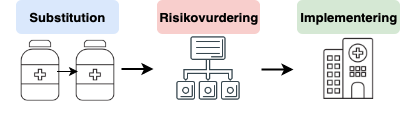
\includegraphics[width=1\textwidth]{billeder/forside.png} \\
		\vspace{3cm}
	 		\begin{Large}
	 		Sundhedsteknologi 3. semester, Master Projekt - Efterår 2018\\
		\vspace{1cm}
			\end{Large}
	{\large Projekt gruppe 18gr9408 \\
	Maria Kaalund Kroustrup}
\end{center}
\vspace*{\fill}

\begin{center}
	\line(1,0){400}
\end{center}




\cleardoublepage												% Indsaetter tom side, saa naeste kapitel starter paa hoejre side (hvis noedvendigt)
\phantomsection
\pdfbookmark[0]{Titelblad}{titelblad}
\thispagestyle{empty}

\begin{minipage}[t]{0.48\textwidth}
\vspace*{-25pt}			%\vspace*{-9pt}

\includegraphics[height=4cm]{billeder/AAU-logo-stud-DK-RGB}
\end{minipage}
\hfill
\begin{minipage}[t]{0.48\textwidth}
{\small 
\textbf{\\ School of Medicine and Health  \\
Biomedical Engineering and Informatics}\\
Niels Jernes Vej 12, 9220 Aalborg Øst \\
http://www.smh.aau.dk}

\end{minipage}

\vspace*{1cm}

\begin{minipage}[t]{0.48\textwidth}
\textbf{Titel:} \\[5pt]\bigskip\hspace{2ex}
Risikovurdering af lægemiddelskift

\textbf{Uddannelse og semester:} \\[5pt]\bigskip\hspace{2ex}
Sundhedsteknologi \\ \bigskip\hspace{2ex} 3. semester kandidat

\textbf{Tema:} \\[5pt]\bigskip\hspace{2ex}
Anvendt sundhedsteknologi \\ \bigskip\hspace{2ex}
og informatik

\vspace*{2mm}

\textbf{Projektperiode:} \\[5pt]\bigskip\hspace{2ex}
Efterår 2018  \\ \bigskip\hspace{2ex} September 2018 til December 2018

\textbf{Projektgruppe:} \\[5pt]\bigskip\hspace{2ex}
18gr9408

\textbf{Deltagere:} \\[5pt]\hspace*{2ex}
Maria Kaalund Kroustrup

\vspace*{5mm}

\textbf{Interne vejleder:} \\[5pt]\hspace*{2ex}
Kirstine Rosenbeck Gøeg 

\vspace*{2mm}

\textbf{Eksterne vejleder:} \\[5pt]\hspace*{2ex}
Hanne Plet\\\bigskip\hspace{2ex}


\textbf{Antal sider: XX} \\
\textbf{Antal appendiks: XX} \\ 
\textbf{Afsluttet: XX/12/2018}

\end{minipage}
\hfill
\begin{minipage}[t]{0.483\textwidth}
\textbf{Synopsis}: \\[5pt]
\fbox{\parbox{7cm}{\bigskip\vspace{-0.3cm}
Lægemidler substitueres for at reducere omkostningerne ved sygehusmedicin. Substitution af lægemidler kan medvirke til en øget risiko for fejlmedicinering og derved have patientsikkerhedsmæssige konsekvenser. Implementering af substituerede lægemidler har derfor betydning for forebyggelsen af medicineringsfejl. 

Risikovurderingen af lægemidler inden implementering i klinikken foretages i Region Nordjylland af medarbejdere fra regionens Sygehusapotek. Denne vurdering sker manuelt og er baseret på erfaringer, hvilket gør den sårbar og personafhængig. 

%Ingen videnskabelig litteratur har undersøgt anvendelsen af informationssystemer til forbedring af den nuværende vurdering af lægemiddelskift, men risikovurdering som beslutningsstøtte system er anvendt inden for samme domæne.

Bidraget i dette projekt er at udvikle et regelbaseret system til risikovurdering af lægemiddelskift og evaluere anvendeligheden af systemet. Risikovurderingen foretages ud fra risikofaktorer, som er beskrevet i litteraturen samt ud fra den nuværende vurdering af lægemiddelskift. På baggrund af disse beregnes en risikoscore, der skal anvendes som et hjælpeværktøj til medarbejderne fra Sygehusapoteket i forhold til at skelne mellem, hvornår et lægemiddelskift kræver særligt opmærksomhed ved implementering.

Det konkluderes at et regelbaseret system er anvendeligt til risikovurdering af lægemiddelskift, men at systemet kræver yderligere tilpasning for at kunne forbedre den nuværende vurdering af lægemiddelskift.
\vspace{-0.2cm}\bigskip}}
\end{minipage}

\vfill

{\footnotesize\itshape Rapportens indhold er frit tilgængeligt, men offentliggørelse (med kildeangivelse) må kun ske efter aftale med forfatter.}

% Rapportens indhold er frit tilgængeligt, men offentliggørelse (med kildeangivelse) må kun ske efter aftale med forfatterne.
% The content of the report is freely available, but publication (with source reference) may only take place in agreement with the authors.

%\chapter*{Abstract}
Drug substitution occur in order to save expenditures on medicine. Substitution of drugs contribute to medication errors in the clinic, which can affect the patient safety. The implementation of drug substitutions are important for reducing medication errors. Currently, risk assessment of drug substitution is performed by employees from the hospital pharmacy in region Northern Jutland. This process occurs manually and the assessment is based on experience, which makes it vulnerable and person-dependent. Therefore, the study aimed to develop a rule-based system for risk assessment of drug substitution. The applicability of the system was evaluated by 11 employees from the hospital pharmacy and the performance of the risk assessment was investigated using Receiver Operating Characteristic. The Area Under the Curve indicated a good test for predicting drugs in need for particular attention when implementing substitutions in the clinic. A limitation of the study was found in the use of risk factors and weights. In conclusion, the present study demonstrates, that a rule-based system is applicable for risk assessment of drug substitution, but  there is need for further investigation for to clarify risk factors and weights in order to modify the system and improve the current assessment of drug substitution.  

\cleardoublepage
%\chapter*{Forord}
Denne rapport er et 3. semesters kandidatprojekt på kandidatuddannelsen Sundhedsteknologi (M.sc. Biomedical Engineering and Informatics) på Aalborg Universitet. Projektet er udarbejdet i perioden september 2018 til december 2018 af Maria Kaalund Kroustrup. 

Projektet er udarbejdet med udgangspunkt i det overordnede tema for semesteret "Anvendt sundhedsteknologi og informatik". I studieordningen for uddannelsen fremgår det at fokus er at være i stand til selvstændigt at initiere eller udføre samarbejde inden for disciplinen samt tage ansvar for deres egen faglige udvikling~\citep{Studieordning2011}. 

Dette projekt omhandler udviklingen af et regel-baseret system til risikovurdering af lægemiddelskift med henblik på at opnå en mere effektiv implementering af lægemiddelskift, hvilket kan bidrage til at forebygge medicineringsfejl og forbedre patientsikkerheden. 

Der rettes stor tak til vejleder Kirstine Rosenbeck Gøeg for vejledningen i projektperioden. Yderligere rettes der tak til eksterne vejleder Hanne Plet, Emilie Middelbo Outzen og Lina Klitgaard Larsen for sparring og bidrag til viden inden for sygehusapoteket. Sidst men ikke mindst rettes der tak til samarbejdet med Sygehusapoteket Region Nordjylland. 

\vspace{1.5cm}
\begin{center}
\rule{6cm}{0.4pt} \\
Maria Kaalund Kroustrup \\
\textit{mkrous14@student.aau.dk}
\end{center}
\section*{Læsevejledning}
\textit{I dette afsnit beskrives opbygningen af rapporten, samt hvordan referencer til figurer og tabeller er angivet. Ligeledes beskrives anvendelse af forkortelser og begreber samt angivelse af referencer til litteratur.}

Rapporten påbegyndes i kapitel 1 med en indledning, hvor problemstillinger ved lægemiddelskift tydeliggøres. Disse problemstillinger analyseres i kapitel 2 ved problemanalysen, hvor overordnede problemstillinger identificeres og sammenfattes i en opsummering. Problemanalysen danner grundlag for udformningen af problemformuleringen. Ud fra problemformuleringen udformes kapitel 3, som indeholder metode.  Resultater opnået ud fra metoden fremlægges af kapitel 4. Hvorefter metoden og resultater diskuteres i kapitel 5. For til sidst at konkludere på problemformuleringen i kapitel 6. Efterfølgende er litteratur og appendiks angivet.

Figurer og tabeller er i rapporten angivet efter det pågældende kapitel. Dette vil sige, at den første figur i kapitel 2 er angivet Figur 2.1 og den første tabel i kapitel 2 er angivet Tabel 2.1. Figurtekst er angivet under den tilhørende figur og tabeltekst er angivet over den tilhørende tabel. 

Forkortelser er i rapporten angivet det førstnævnte sted med ordet med efterfølgende forkortelse angivet i parentes, hvorefter forkortelsen er anvendt i rapporten efterfølgende. Forkortelser og begreber, som ikke er yderligere beskrevet i rapporten, er listet nedenfor i alfabetisk rækkefølge.

Kilder er i rapporten angivet efter Vancouver som kildehenvisning, hvilket betyder, at kilderne nummereres fortløbende og angives i firkantet parentes. Hvis en kilde er angivet før et punktum i en sætningen gælder denne for den pågældende sætningen, hvorimod en kilde efter punktum er gældende for hele sektionen.

\begin{table}[H]
%\caption{Forkortelser}
\label{table:forkortelser}
\begin{tabular}{p{4.5cm} p{9.8cm}}
\multicolumn{2}{c}{\cellcolor[HTML]{C0C0C0}\textbf{ FORKORTELSER}} \vspace{0.2cm} \\
\textbf{ATC} &  Anatomisk Terapeutisk Kemisk \vspace{0.2cm} \\
\textbf{ROC} & Receiver Operating Characteristic \vspace{0.2cm} \\
\textbf{SRN} & Sygehusapoteket Region Nordjylland \vspace{0.2cm} \\
%%\textbf{UTH} 
%%& Utilsigtet hændelse \vspace{0.5cm} \\
%%\textbf{RS} & Registreret specialitet \vspace{0.5cm} \\
%%\textbf{IRS} & Ikke-registreret specialist  \vspace{0.5cm} \\
%%\textbf{RADS} & Rådet for anvendelse af dyr sygehusmedicin \vspace{0.5cm} \\
%\textbf{ATC} & Anatomical Therapeutic Chemical \vspace{0.5cm} \\
%  & \vspace{0.5cm} \\
\end{tabular}
\end{table}
\vspace{-0.8cm}

\begin{table}[H]
%\caption{Begreber}
\label{table:begreber}
\begin{tabular}{p{4.5cm} p{9.8cm}}
\multicolumn{2}{c}{\cellcolor[HTML]{C0C0C0}\textbf{BEGREBER}} \vspace{0.2cm}\\
\textbf{Amgros} & Står for indkøb af lægemidler til landets otte sygehusapoteker og opnår besparelser på lægemidler ved at sende disse i udbud~\citep{Amgros2018b}. \vspace{0.2cm} \\
\textbf{Lægemiddelkomitéen} & Tager stilling til godkendelse af lægemidler på hospitalerne og udarbejder relevante retningsgivende dokumenter, som gælder for lægemiddelområdet~\citep{RegionNordjylland2018}. \vspace{0.2cm} \\
\textbf{Medicinrådet} & Udarbejder anbefalinger og vejledninger om lægemidler til de fem regioner~\citep{Medicinradet2018}.\vspace{0.2cm} \\
\textbf{Utilsigtede hændelse} & En begivenhed, som omfatter kendte og ukendte hændelser og fejl inden for sundhedsvæsnet, som ikke skyldes patientens sygdom, og er skadevoldende eller kunne have været skadevoldende~\citep{AalborgKommune2017}. \\
%\textbf{Analoge substitution:} & Lægemidler med forskelligt aktive stof med nogenlunde ensartet klinisk virkning~\citep{DanskSelskabforPatientsikkerhed2009} . \vspace{0.5cm} \\
%\textbf{Generisk substitution:} & Lægemidler med samme aktive stof \vspace{0.5cm} \\
%\textbf{Kontraktskift:} & Kontraktskift mellem leverandør og Amgros ved Amgrosudbud~\citep{DanskSelskabforPatientsikkerhed2009}.  \vspace{0.5cm} \\
%%\textbf{Restordre:} & Efterspørgslen på et lægemiddel overstiger den tilgængelige mængde af lægemiddel.  \vspace{0.5cm} \\
%%\textbf{Bagatelkøb} & Indkøb af lægemidler med en omsætning på under 500.000 kroner årligt. \vspace{0.5cm} \\
%%\textbf{Utilsigtede hændelser} &  Begivenhed, der forekommer i forbindelse med sundhedsfaglig virksomhed, herunder præhospital indsats, eller i forbindelse med forsyning af og information om lægemidler. Omfatter på forhånd kendte og ukendte hændelser og fejl, som ikke skyldes patientens sygdom, og som enten er skadevoldende eller kunne have været skadevoldende, men forinden blev afværget eller i øvrigt ikke indtraf på grund af omstændighederne. %En begivenhed, der forekommer i forbindelse med sundhedsfaglig virksomhed eller forsyning af og information om lægemidler. Utilsigtede hændelser omfatter på forhånd kendte og ukendte hændelser og fejl, som ikke skyldes patientens sygdom og som enten er skadevoldende eller ikke-skadevoldende ved forekomst.  (Sundhedsloven, Kapitel 61 \§ 198)
% \vspace{0.5cm} \\
%%\textbf{Registreret specialitet:} & Lægemiddel registreret og godkendt af lægemiddelstyrelsen~\citep{Laegemiddelinformaion2017}. \vspace{0.5cm} \\
%%\textbf{Ikke-registreret specialist} & Lægemiddel, der aldrig har været godkendt eller afregistreret i Danmark~\citep{Laegemiddelinformaion2017}. \vspace{0.5cm} \\
%%\textbf{Magistrelt lægemiddel} & Lægemiddel fremstillet på et apotek og ikke vurderet af myndighederne i forhold til kvalitet, sikkerhed og effekt~\citep{Laegemiddelinformaion2017}. \vspace{0.5cm} \\
%%\textbf{Merværdi:} & Den ekstra værdi et lægemiddel kan tilbyde sammenlignet med nuværende standardbehandling vurderet ud fra patientrelaterede kriterier som livsforlængelse, alvorlige symptomer og bivirkninger, helbredsrelateret livskvalitet samt ikke-alvorlige symptomer og bivirkninger  \vspace{0.5cm} \\
%\textbf{Standardbehandling} & Lægemidlet indføres som et alment anvendt behandlingstilbud til en patientgruppe\vspace{0.5cm} \\
%& \vspace{0.5cm} \\
%& \vspace{0.5cm} \\
\end{tabular}
\end{table}


%\begin{table}[H]
%%\caption{Beskrivelse??}
%\label{table:beskrivelser}
%\vspace{0.5cm}
%\begin{tabular}{p{4.5cm} p{9.8cm}}
%\multicolumn{2}{c}{\cellcolor[HTML]{C0C0C0}\textbf{TABEL 3 - BESKRIVELSER}} \vspace{0.5cm} \\
%\textbf{Amgros:} & Regionernes lægemiddelorganisation, hvis formål er at sikre forsyning af lægemidler til offentlige hospitaler i Danmark med henblik på at skærpe konkurrencen mest muligt, samtidigt med at kvalitet og patientsikkerhed sikres. \vspace{0.5cm}
%\\ 
%\textbf{Medicinrådet:} & Et uafhængigt råd, der udarbejder anbefalinger i forhold til standardbehandlinger og behandlingsvejledninger om lægemidler til de fem danske regioner. \vspace{0.5cm} \\
%\textbf{Sygehusapoteket:} & Sikre forsyning af lægemidler,
%fremstilling af sygehusspecifikke lægemidler og leverance af klinisk farmaceutiske serviceydelser. \vspace{0.5cm} \\
%\textbf{Lægemiddelstyrelsen} & Kontrollere og godkender lægemiddelvirksomheder og lægemidler på det danske marked samt overvåger bivirkninger ved lægemidler og godkender kliniske forsøg. Beslutter tilskud til lægemidler og fører tilsyn med medicinsk udstyr. Overvåger utilsigtede hændelser med medicinsk udstyr samt udpeger apotekere, tilrettelægger apoteksstrukturen og fører tilsyn med apoteker og detailforhandlere.\vspace{0.5cm} \\
%\textbf{RADS} & Sikrer ensartet anvendelse af dyr medicin på landets sygehus. Fra år 2017 har Medicinrådet overtaget RADS' opgaver og dens fagudvalg. \vspace{0.5cm} \\
%& \vspace{0.5cm} \\
%& \vspace{0.5cm} \\
%& \vspace{0.5cm} \\
%\end{tabular}
%\end{table}







%%%% Indholdsfortegnelse (TOC) %%%%

\phantomsection													% Kunstigt afsnit, som hyperlinks kan 'holde fast i'
\pdfbookmark[0]{Indholdsfortegnelse}{indhold}					% Tildeler en klikbar bookmark til den endelige PDF
\tableofcontents*												% Indholdsfortegnelsen (kaldet ToC) 

%\addtocontents{toc}{\protect\newpage}							% Fremtvinger sideskift i ToC hvis noedvendig (der hvor koden placeres)


\mainmatter														% Hovedindhold - nummereres fra side 1

%%%% Rapportindhold %%%% 										% Rapportindholdet boer IKKE indeholde broedtekst - KUN includede filer!

%% Indledende %%												% Opdel evt. i passende afsnit for overblikkets skyld
\chapter{Initierende problem}
Den stigende andel af ældre, forekomsten og varigheden af kroniske sygdomme samt udviklingen i sundhedsforventninger og teknologier er skyld i stigende sundhedsudgifter i flere europæiske lande~\citep{Ess2003}. I år 2015 brugte Danmark flere sundhedsudgifter end det gennemsnitlige land i Europa~\citep{EU2017}. Siden år 2007 til 2015 har udgifterne til sygehusmedicin steget i gennemsnit  7,8~\% om året~\citep{Sundhed2016}.

For at begrænse udgifterne har Amgros, Regionernes lægemiddelorganisation, siden år 2007 sendt lægemidler i udbud årligt med henblik på at indkøbe lægemidler af høj kvalitet til bedst mulige priser til de offentlige danske hospitaler~\citep{Sygehusapoteket2017}. Udbud forekommer på lægemidler, hvor der findes mere én leverandør, hvormed lægemidler bringes i konkurrence. Ved levering af lægemidler fra en ny leverandør sker et 
kontraktskift~\citep{Amgros2015}. Foruden kontraktskift kan lægemiddelskift forekomme ved restordre, hvor efterspørgselen på et lægemiddel overstiger den tilgængelige mængde~\citep{Amgros2015}. Restordre kan skyldes leveringesvigt fra leverandøren eller producenten og det er i disse tilfælde leverandørens ansvar at finde et erstatningslægemiddel~\citep{Laegemiddelinformaion2017, Amgros2017}. 

Et lægemiddelskift kan defineres som simple eller kompleks i forhold til hvordan det påvirker afdelingen~\citep{Laegemiddelinformaion2017, Sygehusapoteket2017a}. Et simpel lægemiddelskift påvirker klinikken i lav grad og sker dagligt i forbindelse med skift til et simpel generisk lægemiddel.%Generisk lægemiddel indeholder samme aktive stof som det nuværende lægemiddel, men indeholder andre hjælpemidler. 
Hvorimod et kompleks lægemiddelskift påvirker klinikken i større grad og omhandler komplekse generiske lægemiddelskift, hvor der er flere ændringer som f.eks. styrke og disponeringsform afviger fra det nuværende lægemiddel.~\citep{Laegemiddelinformaion2017, Sygehusapoteket2017a}

Implementering af lægemiddelskift i klinikken skaber økonomiske og patientsikkerhedsmæssige udfordringer der kan lede til en utilsigtede hændelser (UTH'er)~\citep{Laegemiddelinformaion2017, Sygehusapoteket2017a}. De hyppigste årsager til UTH'er skyldes i år 2013 medicinering~\citep{Patientombuddet2013}. Af 824 rapporterede UTH'er i Region Nordjylland skyldes 97~\% medicinering 86~\% administration af medicin og 41~\% at intet medicin var givet til patienten~\citep{Jensen2014}

Rapportering af UTH'er har foruden at synliggøre problemstillinger dannet grundlaget for at forbedre og forebygge med henblik på at nedbringe antallet af rapporterede UTH'er~\fxnote{Find kilde}. Elektronisk beslutningsstøttesystem, stregkode scanning og klar-til-brug lægemidler har medført en reduktion i antallet af medicineringsfejl internationalt og nationalt~\citep{Bates2013, Levtzion-korach2010, Amgros2012}.  

På baggrund af dette er det relevant at analysere, hvilke problemstillinger der opstår i forbindelse med lægemiddelskift med henblik på at undersøge, hvorledes disse problemstillinger kan anvendes i en algoritme til at forudsige og derved forebygge antallet af UTH'er.

%\citep{Bates2013, Cheng2011, Raboel2005, Poon2006, Bates2000,Levtzion-korach2010,Oren2003, Amgros2012}. 

%I periode fra 2007 til 2015 har udgifterne til sygehusmedicin steget i gennemsnit med 7,8~\% om året, hvilket svarer til en stigning på 3,5 milliarder kroner over en periode på 8 år ~\citep{Sundhed2016}.Dette er til trods for at Amgros, Regionernes lægemiddelorganisation, årligt sender lægemidler i udbud med henblik på at indkøbe de rigtige lægemidler til den bedst mulige pris til de offentlige danske hospitaler~\citep{Sygehusapoteket2017}. Udbuddene forekommer på lægemidler hvor der findes mere én leverandør, på denne måde bringes lægemidlerne i konkurrence, hvilket kan give anledning til kontraktskift~\citep{Amgros2015}.

%Foruden kontraktskift kan lægemiddelskift forekomme ved restordre, hvor efterspørgselen på et lægemiddel overstiger den tilgængelige mængde~\citep{Amgros2015}. Dette kan skyldes leveringesvigt fra leverandøren eller producenten og det er i disse tilfælde leverandørens ansvar, grundet kontrakten, at finde et erstatningslægemiddel~\citep{Laegemiddelinformaion2017, Amgros2017}. 

%Ved implementering af lægemiddelskift er der både økonomisk og patientsikkerhedsmæssige problematikker som kan påvirke afdelingen fra lav til mellem eller høj grad~\citep{Laegemiddelinformaion2017, Sygehusapoteket2017a}. Studie har vist at de hyppigste utilsigtede hændelser ved lægemidelskift omhandler fejlmedicinering~\citep{Hakonsen2010}. Yderligere er antallet af rapporterede utilsigtede hændelser i Region Nordjylland steget med over 36~\% fra år 2012 til 2014~\citep{Jensen2014}.


%% Problemanalyse %%
\include{intro/ProblemanalyseNEWNEW}
%\section{Lægemiddelskift}
Lægemiddelskift forekommer når en ny lægemiddelvirksomhed vinder leverancen af nyt lægemiddel som standardbehandling, hvormed der er indgås et kontraktskift~\citep{Amgros2015}. 

Forinden et kontraktskift kan forekomme analyseres og vurderes lægemidlet i samarbejde med Medicinrådet og Amgros~\citep{DanskeRegioner2016}, som beskrevet i Appendiks \ref{cha:AppA}. Efter analyseringen og vurdering sendes lægemidlerne i udbud via Amgros med henblik på at indkøbe lægemidler af høj kvalitet til bedst mulige pris~\citep{Sygehusapoteket2017}.

Størstedelen af lægemidler i ATC-grupper sendes i udbud en gang årligt fra start september til midt november, hvor udbud på ATC-grupper som indgår i Medicinrådets behandlingsvejledninger sker løbende hen over året~\citep{Sygehusapoteket2017}, som beskrevet i Appendiks \ref{cha:AppD}.
Forinden udbuddet defineres antallet af vindere samt, hvorvidt udbuddet skal bygge på laveste pris eller være mest økonomisk fordelagtigt~\citep{Amgros2018a}, som beskrevet i Appendiks \ref{cha:AppB}.

På baggrund af de foregående analyser og vurderinger fastsættes et prisniveau der anvendes som beslutningsgrundlag for Medicinrådet om, hvorvidt lægemidlet skal anvendes som standardbehandling~\citep{DanskeRegioner2016}. Hvis standardbehandlingen er det eneste lægemiddel inden for terapiområdet kan dette implementeres direkte på hospitalet. I tilfælde af flere lægemidler inden for samme terapiområde, skal lægemidlernes ligeværdighed vurderes af Medicinrådet, som beskrevet i Appendiks \ref{cha:AppA}, med henblik på at udarbejde behandlingsvejledninger og rekommendationer for lægemidlerne. Disse videresendes til de danske hospitaler, som står for implementeringen.~\citep{DanskeRegioner2016}

Kontraktskift medfører substitution af lægemidler, hvor et lægemiddel udskiftes til et andet~\citep{DanskSelskabforPatientsikkerhed2009}. Der findes to typer af substitution herunder analog og generisk.
Analog substitution omhandler lægemidler der indeholder forskelligt aktivt lægemiddelstof, har nogenlunde ens effekt og bivirkninger. Disse kræver ændring i ordination og skal derfor ordineret af en læge. Generisk substitution omhandler lægemidler som indeholder det samme virksomme lægemiddelstof og fungere derfor som hinandens synonyme. Dette skift kræver ikke en ændring i recept og kan derfor varetages af en sygeplejerske.~\citep{DanskSelskabforPatientsikkerhed2009}

Et simpelt lægemiddelskift er vurderet til at påvirke hospitalsafdelingen i lav grad og varetages logistik afdeling~\citep{Laegemiddelinformaion2017, Sygehusapoteket2017a}. Disse skift sker dagligt i forbindelse med et simpel generisk lægemiddelskift. Hvorimod et kompleks lægemiddelskift påvirker klinikken i mellem til høj grad og kræver ofte involvering af flere interessenter som f.eks. medicinansvarlig, overlæger, kontaktsygeplejersker eller medicinservicefarmakonomer til at undersøge lægemidlets anvendelighed for det pågældende hospitalsafsnit. 
De komplekse skift sker ved generiske lægemidler, hvor flere faktorer som f.eks. styrke og disponeringsform afviger fra den nuværende behandling.~\citep{Laegemiddelinformaion2017,Sygehusapoteket2017a}

%\section{Implementering af nyt lægemiddel}
Forinden et lægemiddel kan implementeres indkøbes lægemidlerne af Sygehusapoteket Region Nordjylland (SRN) som står for indkøb af lægemidler til distribution på de Nordjyske hospitaler ~\citep{SygehusapoteketRegionNordjylland2013}, som beskrevet i Appendiks \ref{cha:AppC}. Implementering af lægemidlet vurderes af ATC-ansvarlige, som er eksperter på området, som simpel eller kompleks på baggrund af flere faktorer~\citep{Sygehusapoteket2017}, som er beskrevet i Appendiks \ref{cha:AppD}. Dette indebærer f.eks. risikovurdering på afsnittet og lægemidlet samt type skift herunder bl.a. skift af dosis eller device og analoge lægemidler~\citep{Sygehusapoteket2017}. 

Et simpelt lægemiddelskift er vurderet til at påvirke klinikken i lav grad og varetages ofte af SRN's logistik afdeling~\citep{Laegemiddelinformaion2017, Sygehusapoteket2017a}. Disse skift sker dagligt i forbindelse med et simpel generisk lægemiddelskift. Hvorimod et kompleks lægemiddelskift påvirker klinikken i mellem til høj grad og kræver ofte involvering af flere interessenter som f.eks. medicinansvarlig, overlæger, kontaktsygeplejersker eller medicinservicefarmakonomer til at undersøge lægemidlets anvendelighed for det pågældende hospitalsafsnit. 
De komplekse skift sker ved generiske lægemidler, hvor flere faktorer som f.eks. styrke og disponeringsform afviger fra den nuværende behandling.~\citep{Laegemiddelinformaion2017,Sygehusapoteket2017a}

%
\section{Problemstillinger ved lægemiddelskift}
%Lægemiddelskift medvirker til reportering af utilsigtede hændelser (UTH'er)~\citep{Amgros2015}.
%Et præparatskift giver øgede administrative og kliniske udgifter og kan i værste fald betyde fejlmedicinering af patienter.
%http://www.amgros.dk/media/1589/Amgros%20Årsmagasin.pdf

De hyppigste årsager til UTH'er på de danske hospitaler skyldes i år 2013 medicinering, hvilket udgjorde 23,97~\%.~\citep{Patientombuddet2013}. Antallet af rapporterede UTH'er i Region Nordjylland er steget med over 36\% fra år 2012 til 2014 ~\citep{Jensen2014}. Ud af 824 rapporterede UTH'er i år 2014 omhandlede 97\% af disse medicinering, 86\% administration af medicin og 41\% disponering~\citep{Jensen2014}. Det er i flere studier undersøgt de utilsigtede hændelser forårsaget af henholdsvis ordinationer, dispensering og administration af medicin, hvilket fremgår af tabel \ref{table:UTHordination}, \ref{table:UTHdispensering} og \ref{table:UTHAdministration}. En fælles årsag til de rapporterede UTH'er er forkert dosis, forkert lægemiddel og udeladelse af henholdsvis ordination, dispensering og administration.

	\vspace{2mm}
\begin{longtable}{p{5cm}|p{4.2cm}|p{2cm}|p{2cm}}
	\caption{Utilsigtede hændelser ved ordinationer.}
	\vspace{2mm}
	\label{table:UTHordination} \\
\cellcolor[HTML]{C0C0C0} {\textbf{Årsager}} & 
{\cellcolor[HTML]{C0C0C0}\textbf{Sundhedsstyrelsen~\citep{Sundhedsstyrelsen2005}}} &
{\cellcolor[HTML]{C0C0C0}\textbf{Lisby et al~\citep{Lisby2005}}} &
{\cellcolor[HTML]{C0C0C0}\textbf{Tully et al~\citep{Tully2009}}} \\ \hline
%{\cellcolor[HTML]{C0C0C0}\textbf{4}} 
%\textbf{Metode} & Gennemgang af indberettede UTH'er & Observation, stikprøvekontrol, journalgennemgang & Gennemgang af medicinlister & Gennemgang af indberettede UTH'er \\ \hline
Forkert dosis & - & - & 12,5~\%  \\ \hline %& 29,6      \\ \hline
Forkert lægemiddel & 16,3~\% & - & - \\ \hline % & 14,5 \\ \hline
Forkert patient & 3,8~\% & - & - \\ \hline %& 11,2 \\ \hline
Intet lægemiddel ordineret & 20,7~\% & - & 15,9~\% \\ \hline % & 24,1 \\ \hline
Udeladelse af formulering & - & 38,0~\% & - \\ \hline %& - \\ \hline
Udeladelse af administrationsvej & - & 34,7~\% & - \\ \hline %& - \\ \hline
Udeladelse af doseringstidspunkt & - & 10~\% & 10,4*~\% \\ \hline %& - \\ \hline
Manglende angivelse af maskimal dosis & - & - & 12,1~\% \\ \hline %& -  \\ \hline
Overset kontraindikation & 14,3~\% & - & 0,3~\% \\ \hline %& 19,6 \\ \hline
\cellcolor[HTML]{C0C0C0} {\textbf{Total antal fejl}} & 
{\cellcolor[HTML]{C0C0C0}\textbf{526}} &
{\cellcolor[HTML]{C0C0C0}\textbf{320}} &
{\cellcolor[HTML]{C0C0C0}\textbf{3455}}
\end{longtable}

Ud fra tabel \ref{table:UTHordination} fremgår det at de hyppigste årsager til UTH ved ordinationer skyldes 38~\% af de 320 rapportede UTH'er udeladelse af formulering og 34,7~\% administrationsvej~\citep{Lisby2005}. To studier påviste at i 20,7~\% ud af 526 og 15,9~\% af 3455 skyldes at intet lægemiddel var ordineret~\citep{Sundhedsstyrelsen2005, Tully2009}. Årsager som intet lægemiddel ordineret, udeladelse af doseringstidspunkt samt overset kontraindikation er dokumenteret af flere studier~\citep{Sundhedsstyrelsen2005, Lisby2005, Tully2009}. 

\vspace{2mm}
\begin{longtable}{p{5cm}|p{4.2cm}|p{2cm}|p{2cm}}
	\caption{Utilsigtede hændelser ved dispensering.}
	\vspace{2mm}
	\label{table:UTHdispensering} \\
\cellcolor[HTML]{C0C0C0} {\textbf{Årsager}} & 
{\cellcolor[HTML]{C0C0C0}\textbf{Sundhedsstyrelsen~\citep{Sundhedsstyrelsen2005}}} &
{\cellcolor[HTML]{C0C0C0}\textbf{Lisby et al~\citep{Lisby2005}}} &
{\cellcolor[HTML]{C0C0C0}\textbf{Barker et al~\citep{Barker2002}}} \\ \hline
%\textbf{Metode} & Gennemgang af indberettede UTH'er & Observation, stikprøvekontrol, journalgennemgang & Gennemgang af medicinlister & Gennemgang af indberettede UTH'er \\ \hline
Forkert dosis & 26,6~\% & 29,4~\% &  20,0~\% \\ \hline
Forkert lægemiddel & 52,2~\% & - & - \\ \hline
Forkert tidspunkt & - & 1,1~\% & 40,3~\% \\ \hline
Udeladt dispensering & 11,4~\% & 41,2~\% & 27,9~\% \\ \hline
%Dispensering af et
Ikke ordineret lægemiddel & - & 29,4 & 4,8 \\ \hline
\cellcolor[HTML]{C0C0C0} {\textbf{Total antal fejl}} & 
{\cellcolor[HTML]{C0C0C0}\textbf{184}} &
{\cellcolor[HTML]{C0C0C0}\textbf{17}} &
{\cellcolor[HTML]{C0C0C0}\textbf{290}}
\end{longtable}

Ud fra tabel \ref{table:UTHdispensering} fremgår det at de hyppigste årsager til UTH ved dispensering skyldes i 52,2~\% af de 184 rapporterede UTH'er forkert lægemiddel. Udover forkert lægemiddel blev der påvist forkert dosis, forkert tidspunkt eller udeladelse af dispensering samt ikke ordineret lægemiddel, hvor dette er dokumenteret i flere af studierne som værende en årsag til rapporteret UTH'er~\citep{Lisby2005, Sundhedsstyrelsen2005,Barker2002}.

\vspace{2mm}
\begin{longtable}{p{5cm}|p{4.2cm}|p{2cm}|p{2cm}}
	\caption{Utilsigtede hændelser ved administration.}
	\vspace{2mm}
	\label{table:UTHAdministration} \\
\cellcolor[HTML]{C0C0C0} {\textbf{Årsager}} & 
{\cellcolor[HTML]{C0C0C0}\textbf{Sundhedsstyrelsen~\citep{Sundhedsstyrelsen2005}}} &
{\cellcolor[HTML]{C0C0C0}\textbf{Lisby et al~\citep{Lisby2005}}} &
{\cellcolor[HTML]{C0C0C0}\textbf{Barker et al~\citep{Barker2002}}} \\ \hline
%\textbf{Metode} & Gennemgang af indberettede UTH'er & Observation, stikprøvekontrol, journalgennemgang & Gennemgang af medicinlister & Gennemgang af indberettede UTH'er \\ \hline
Forkert dosis & 37,5~\% & - & 20,0~\% \\ \hline
Forkert lægemiddel & 19,1~\% & - & - \\ \hline
Forkert tidspunkt & 8,9~\% & - & 40,3~\% \\ \hline
Forkert patient & - & 15,7~\% &  - \\ \hline
Udeladt administration & 15,0~\% & - & 27,9~\% \\ \hline
Manglende identifikation af patient & - & 78,9~\% & - \\ \hline
\cellcolor[HTML]{C0C0C0} {\textbf{Total antal fejl}} & 
{\cellcolor[HTML]{C0C0C0}\textbf{839}} &
{\cellcolor[HTML]{C0C0C0}\textbf{190}} &
{\cellcolor[HTML]{C0C0C0}\textbf{290}}
\end{longtable}
\vspace{0.25cm}

Ud fra tabel \ref{table:UTHAdministration} fremgår det at de hyppigste årsager til UTH ved administration i 78,9~\% af de 190 rapporterede UTH'er manglende patientidentifikation~\citep{Lisby2005}. I et af studierne skyldes 40,3~\% ud af 290 af tilfældene forkert tidspunkt~\citep{Barker2002} og i 37,5~\% af 839 forkert dosis~\citep{Sundhedsstyrelsen2005}. Forket dosis, forkert tidspunkt og udeladt administration var dokumenteret i flere studier~\citep{Lisby2005,Sundhedsstyrelsen2005,Barker2002}.

\subsection{Utilsigtede hændelser ved kontraktskift}
De patientsikkerhedsmæssige konsekvenser opstået ved kontraktskift er undersøgt af et norsk studie~\citep{Hakonsen2010}. Interview med 100 sygeplejersker påviste at der opstod fejlmedicinering ved generiske lægemidler. Fejl i ordination og manglende dokumentation af lægemiddelskift foretaget af lægen blev opdaget af 46~\% sygeplejersker dagligt, hvorimod sygeplejerskerne altid fik lægemiddelsiftet dokumenteret. Yderligere følte 92~\% af sygeplejerskerne at generiske lægemidler var tidskrævende og 91~\% at disse øgede risikoen for fejl ved disponering.~\citep{Hakonsen2010}. De typiske hændelser ved kontraktskift fremgår af Figur \ref{fig:UTHkontraktskift}.

\begin{figure}[H]\centering
	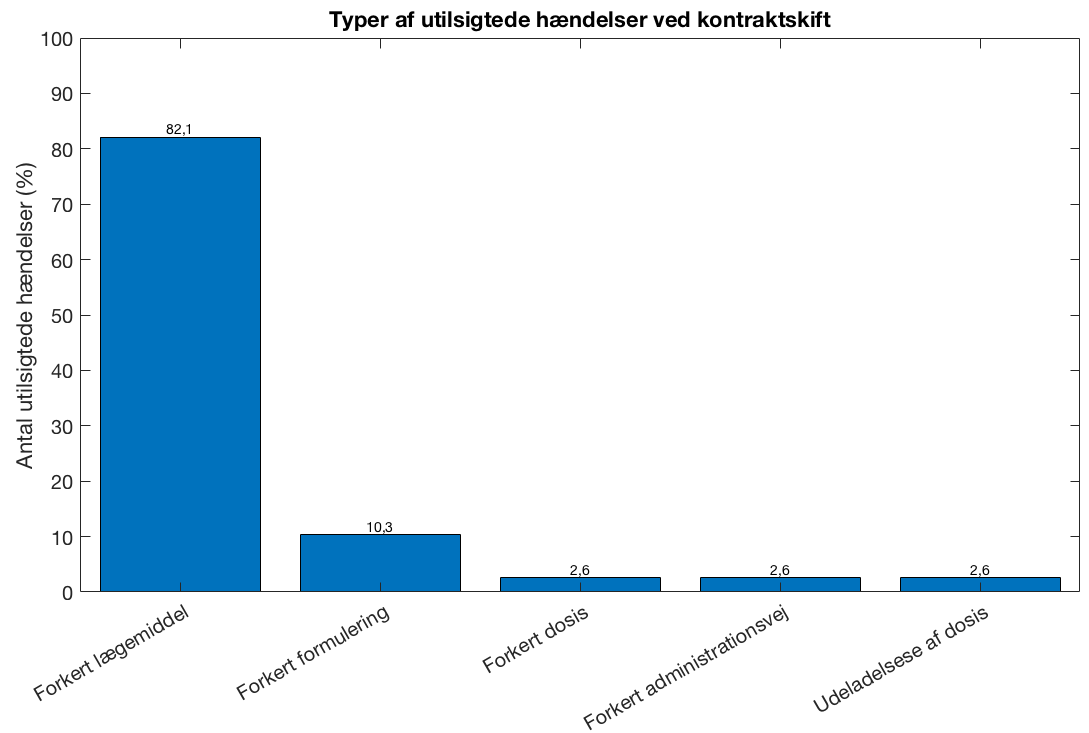
\includegraphics[width=1\textwidth]{billeder/UTH1.png} 
	\caption{Utilsigtede hændelser opstået ved kontraktskift\citep{Hakonsen2010}.}
	\label{fig:UTHkontraktskift}  
\end{figure}

Af Figur \ref{fig:UTHkontraktskift} fremgår det at 82,1~\% af UTH'erne forekommer ved disponering af forkert lægemiddel. Den næst hyppigste er forkert formulering hvor 10,3\% af UTH'er er berettiget mod dette. I  sjældnere tilfælde sker forkert dosis, administrationsvej samt udeladelse af dosis. 

\subsection{Utilsigtede hændelser ved restordre}
Studie har påvist at restordre påvirker patientsikkerheden ved anvendelse af generisk lægemiddel eller manglende alternativ behandling~\citep{Baumer2004}. Gennem spørgeskemaundersøgelse besvaret af farmaceuter blev UTH'er identificeret ved restordre. Undersøgelsen skelner mellem opståede hændelser og nærhændelser, som kunne være opstået~\citep{McLaughlin2013,McBride2013}. Typer af UTH'er identificeret ved restordre fremgår af figur \ref{fig:UTHrestordre}. 


\begin{figure}[H]\centering
	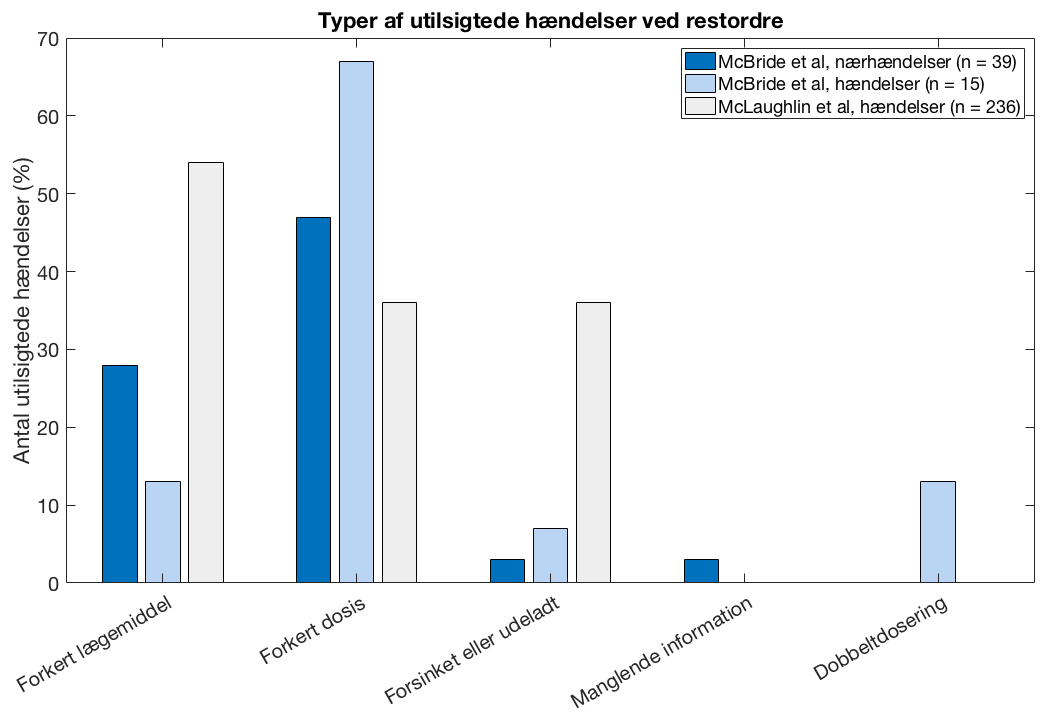
\includegraphics[width=1\textwidth]{billeder/UTH2.png} 
	\caption{Utilsigtede hændelser opstået ved restordre~\citep{McLaughlin2013,McBride2013}.}
	\label{fig:UTHrestordre}  
\end{figure}

Ud fra figur \ref{fig:UTHrestordre} fremgår det at forket dosis af lægemiddel og forsinket dosis var den hyppigste årsag til UTH'er ved restordre~\citep{McLaughlin2013,McBride2013}. Yderligere blev der i studierne identificeret UTH'er ved forsinket eller udeladt dispensering og administrering. Manglende information og dobbeltdosering blev påvist i et af studierne som en årsag til UTH'er ved restordre.~\citep{McLaughlin2013,McBride2013}
%\section{Forebyggelse af problemstillinger ved lægemiddelskift}
Den europæiske lægemiddelstyrelse har udviklet guidelines med henblik på at forebygge problemer opstået ved forveksling af lægemidler og derved reducere antallet af medicineringsfejl~\citep{DanskSelskabforPatientsikkerhed2009}. Disse guidlines er ikke indført i Danmark, men der har været fokus på problemer med emballage forvekslinger, hvormed lovgivningen i Danmark er at pakninger ikke må kunne forveksles.   

Udover guidelines har internationle studier påvist at stregkode teknologi reducerer antallet af fejl i medicineringsprocessen~\citep{Poon2006, Levtzion-korach2010} Stregkode teknologi kan anvendes til at sikre at den rette medicin modtages af den rette patient~\citep{Amgros2013}.  
Amgros har siden år 2010 stillet krav til stregkode på yderste og inderste emballage på lægemidler~\citep{Amgros2013}. Foruden at undgå alvorlige medicinrelaterede fejl kan stregkoder medfører en mere enkel og sikker registrering af lægemiddel i patienternes medicinjournal og effektiv tilbagekaldelse af medicin via it-systemer~\citep{Amgros2013}. Implementering af stregkode teknologi er påvirket af manglende stregkoder og dokumentation ved generisk lægemiddel~\citep{Amgros2013}.

Det anbefales yderligere at anvende store og små bogstaver til navne på lægemidlerne i flere lande med henblik på at advare sundhedspersonalet om lignende lægemidler~\citep{ISMP2011,HQSC2013,ACSQ2011}. Sundhedspersonalet vurderede at det vil have en gavnlig effekt at blive advaret via Tall Man Lettering og at dette især vil have en betydning for lægemidler, hvor navneforveksling kan opstå~\citep{Campmans2018}.

Ligeledes har klinisk besluningstøtte i forhold til advarsler ved forveksling af navn og styrke vist sig at have en positiv effektiv i forhold til at forebygge antallet af medicineringsfejl~\citep{Campmans2018}. Flere studier har påvist at implementering af elektronisk beslutningsstøtte reducerer antallet af fejl~\citep{DW1998,Bates2013,Cheng2011,Raboel2005} og beskrives som et vigtigt redskab til at øge kvaliteten af medicinering med henblik på at nedbringe fejl~\citep{Raboel2005}. Klinisk beslutningsstøtte er anvendt i vid udstrækning inden for sundhedssektoren som f.eks. ved kontrol af lægemiddelallergier og interaktioner mellem to eller flere lægemidler~\citep{Raboel2005}. 
%\section{Problemafgræsning}
På trods af at lægemidlerne sendes i udbud via Amgros med henblik på at opnå økonomiske besparelser er sundhedsudgifter til sygehusmedicin stigende. Udover det økonomiske aspekt medvirker implementeringen af lægemiddelskift til patientsikkerhedsmæssige konsekvenser på grund af medicineringsfejl. Størstedelen af fejlene forekommer ved forkert lægemiddel ved generisk substitution og de hyppigeste årsager til dette skyldes lignende og/eller svært navn på lægemidlet. Guidelines er udviklet med henblik på at undgå forveksling af navn samt emballage på lægemidlerne. Stregkode teknologier har påvist at have gavnlige effekter ved at reducere antallet af medicineringsfejl. Ligeledes er klinisk beslutningssøtte, som er anvendt i vid udstrækning inden for sundhedssektoren, påvist i flere studier at medvirke til reduceringen af fejl og anses samtidig som et vigtigt redskab til at øge kvaliteten ved medicinering.

\section{Problemformulering}
\textit{Hvilket potentiale har en algoritme som beslutningsstøttesystem til kategorisering af lægemidler med henblik på at forebygge fejl ved medicinering?}



\chapter{Problemanalyse}
\textit{I dette kapitel analyses problemstillinger, som opstår i forbindelse med lægemiddelskift. Disse problemstillinger vil sammenfattes i en opsummering og afsluttes med en problemformulering, der danner fremadrettet grundlaget for rapporten.}

\section{Typer af lægemiddelskift}
Lægemiddelskift kan forekomme i forbindelse med kontraktskift eller ved restordre~\citep{Amgros2015}. Et årligt udbud foretages af Amgros, hvis der findes mere end én leverandør af lægemiddelet. På denne måde bringes lægemidlerne i konkurrence, hvilket kan medføre et kontraktskift. I tilfælde af patent på lægemidlet er der ikke analog konkurrence, da prisen på lægemidlet ofte er fastsat. Restordre forekommer når efterspørgslen på et lægemiddel overstiger den tilgængelige mængde.~\citep{Amgros2015}. Udover kontraktskift og restordre kan bagatelkøb medføre præparatskift. Ved bagatelkøb er sygehusapoteket ikke forpligtet til at anvende lægemidlet og leverandøren omfattes ikke af indkøbs- eller forsyningspligt~\fxnote{\url{https://levportal.amgros.dk/Udbudsoversigt/Sider/Bagatelkob.aspx}}

\subsection{Kontraktskift}
Før et udbud finder sted har Amgros en dialog med medicinrådet~\citep{Amgros2017, Amgros2017a}. Lægemidlerne vurderes i forhold til effekt, eksisterende behandling og pris med det formål at stræbe efter laveste priser samt bedst mulig behandling for patienterne. Medicinrådet kategoriserer nye lægemidler og indikationer i forhold til den nuværende standardbehandling i stor, vigtig, lille eller ingen merværdi. Ud fra dette sammenstiller Amgros standardbehandlingen over for en omkostningsanalyse, der er udarbejdet af ansøgeren for lægemiddelskift. Amgros vurderer, hvorvidt de tilsendte oplysninger er relevante og valide. Den kliniske merværdi, omkostningsanalyse og estimeringen af budget konsekvenser danner grundlaget for prisforhandling. Medicinrådet beslutter efter prisforhandlingen, hvorvidt det nye lægemiddel skal anvendes som standardbehandling. Hvis dette er tilfældet foretages et kontraktskift.~\citep{Amgros2017, Amgros2017a}

\subsection{Restordre}
Restordre kan forekomme på forskellige måder som f.eks. leveringesvigt, mangel på råvarer, forhindring i produktion, større forbrug af lægemidlet end beregnet eller at lægemidlet er solgt til en højere pris til et andet land~\citep{Amgros2017}. I tilfælde af restordre er det leverandørens ansvar at dække hospitalsapotekernes udgift ved indkøb af et erstatningslægemiddel~\fxnote{\url{https://levportal.amgros.dk/SiteCollectionDocuments/1.\%20Grundl\%C3\%A6ggende\%20information\%20om\%20l\%C3\%A6gemiddeludbud.pdf}}.


\section{Problematikker ved lægemiddelskift}
Der er både økonomiske og patientsikkerhedsmæssige konsekvenser ved et lægemiddelskift....

\subsection{Kontraktskift}

\subsection{Restordre}
Det er omkostningsfuldt når et lægemiddel går i restordre, da arbejdsgangen på hospitalsafdelingerne skal justeres~\citep{Amgros2015}. Der skal f.eks. foretages vareskift i systemer, på lagre og i medicinrum. Yderligere skal der gives behandlingsinstruktioner til hospitalsafdelingerne. Udover de økonomiske faktorer udgør restordre patientsikkerhedsmæssige risici. Der kan opstå utilsigtede hændelser (UTH'er), hvis præparatet har skiftet navn, udseende og håndteringen af medicin er ændret. Disse risici kan mindskes ved instrukser og ændring af procedure på hospitalerne.~\citep{Amgros2015}


\section{Løsningsstartegier ved lægemiddelskift}

\subsection{Kontraktskift}

\subsection{Restordre}

*** SE 19Præparat ***

%% Kontekst %%
\chapter{Metode}
\textit{I dette kapitel beskrives de metoder som er anvendt til udvikling af en algoritme til kategorisering af  lægemiddelskift.}

\section{Udviklingstrin}
I udviklingsprocssen gennem gås forskellige step hvilket fremgår af Figur \ref{fig:XXX}

\begin{figure}[H]\centering	
\includegraphics[width=0.5\textwidth]{billeder/Black_box.png} 
	\caption{XXXX.}
	\label{fig:XXX}  
\end{figure}

\section{Dataindsamling}
Indsamlet data omhandler Amgrosskift i år 2017. Disse data er enten indsamlet af Amgros eller af Sygehusapoteket Region Nordjylland (SRN) i forbindelse med lægemiddelskift. Data fra Amgros omfatter Amgrosskift fra år 2018 (Amgros2018)~\fxnote{Jeg har brug for at få data fra 2017 i stedet, da dette passer til det andet excel eller så skal jeg have et opdateret med amgrosskift i år 2018}. Data fra SRN omfatter amgrosskift fra år 2017\fxnote{OBS!} (SRN2018) og problemstillinger vedrørende amgrosskift (Problem), som omfatter dokumenteret problemstillinger fra år 2012 til 2017. Alt data er indsamlet i excelark, den opsamlede data kan ses af \ref{table:XXX}

\vspace{2mm}
\begin{longtable}{p{2.5cm}|p{1cm}|p{11cm}}
	\caption{**DET HER ER KUN TIL MIG SELV**}
	\vspace{2mm}
	\label{table:XXX} \\
\cellcolor[HTML]{C0C0C0} {\textbf{Data}} & {\cellcolor[HTML]{C0C0C0}\textbf{Antal}} & 
{\cellcolor[HTML]{C0C0C0}\textbf{Indhold}} \\ \hline
Amgros & 245 & Kontrakt start, ATC-kode, Varenummer 2017, Lægemiddel 2017, Dispenseringsform 2017, Styrke 2017, Pakningsstørrelse 2017, Varenummer 2018, Lægemiddel 2018, Dispenseringsform 2018, Styrke 2018, Pakningsstørrelse 2017, Bemærkning, Rekommenderet.\\ \hline
SRN & 5397 & ATC-koder, Matchstatus, Generisk navn, Firma, Varenummer, Forv. Varenummer, SA-Gl.Vnr (Kig Amgros estimering), Varenummerskift – 1 er skift 0 fortsætter (Kig Amgros estimering), Varenavn, Disponeringsform, Styrke, Pakning, Udbudsgruppe, Udbudsnummer (1-730), Vinder (1, 2, 3, 4, 5, 1x, 2x, BA, k), RADS-MR (0, 1) (RADS- medicin rådet måske medicinrådet??), Amg. Est., Budget pakning, Rev. Pakning, Bemærkning, SAIP/Pakning, AIP/Pakning,
AIP/Enhed, Enh./Paking , Budget slut, Indkøb start, Indkøb slut, Leadtime, Ingen prisvisning, Modified, ID, Created.\\ \hline
Problem & 103 & ATC-kode, Generisk navn, Firma, Varenummer, Varenavn, Udbudsgruppe, Udbudsnummer, Vinder, Debitor, Problemstilling/Bemærkning, Konsekvens, Simpel SAID-sag oprettet, Udfyldt af, Dato. \\ \hline
\end{longtable}



\section{Metode baggrund}
Der er to typer af mashine learning herunder unsupervised og supervised, da input-output relationer er kendt anvendes supervised machine learning. Inden for supervised learning anvendes kategorisering eller regression. Kategorisering identificerer en ny observation til et sæt af kategorier på baggrund af et træningssæt af data, hvor outputtet er kendt. Et eksempel på dette kan være at tildele en diagnose til en given patient baseret på patientens observerede egenskaber som f.eks. køn, blodtryk, tilstedeværelse eller fravær af visse symptomer. 

De enkelte observationer er ofte analyseret i et sæt kvantificerbare egenskaber, som er kendt forskelligt som forklarende variabler. Disse variabler kan have forskellige kategorier f.eks. stor, medium eller lille. Det kan også være antallet af forekomster af et  bestem ord. Andre klassifikationer arbejder med at sammenligne observationer til tidligere observationer ved brug af lighed og afstandsfunktioner.

En algoritme med disse egenskaber betegnes som en klassifikator, som henviser til den matematiske funktion, implementeret af en klassifikationsalgoritme, som kortlægger input til en kategori.

I maskinlæring er observationerne ofte kendt som forekomster, de forklarende variabler betegnes funktioner (grupperet i en funktionsvektor), og de mulige kategorier, der skal forudsiges, er klasser. 

\section{Regel-baseret system}
Tænkning i fakta og regler er måske en af ​​de mest almindelige måder at nærme sig problem definition og problemløsning både i hverdagen
liv og under mere formelle omstændigheder.
Det ønskes at udarbejde et regel-baseret system som kan gemme og manipulere viden til at fortolke information på en nyttig måde. Er adopteret fra artificial intelligence (AI) og knowledge engineering (KE). Regel-baseret systemer er sæt af regler, der efterligner logiske konsekvenser. Regel-baserede systemet udgør et kraftfuldt værktøj til specifikation af viden inden for design og implementering af vidensbaserede systemer (KBS) inden for anvendt kunstig intelligens og vidensteknik. 

Logiske regler
er dem defineret af mennesket; de er normalt subjektive, lokale, kan ændres
Hvis det er nødvendigt. Selvom regelbaserede systemer er et værktøj allestedsnærværende inden for videnskab, teknologi
og hverdagen er deres kodning, analyse og design sjældent et spørgsmål om
dybere teoretisk undersøgelse I de fleste af applikationsområderne bruges de netop (bevidst eller ubevidst) på en retfærdig måde, anvendt til at løse specifikt problem uden at være opmærksom på spørgsmål som deres egenskaber,
sprog, optimering osv. Selvom regelbaseret indledning ikke er
Den eneste mulighed for argumentation, logiske systemer er for det meste konstrueret som
sammensat af aksiomer (fakta) og indledning regler.

RBS til kontrol eller beslutningsstøtte
består af et enkeltlags sæt regler og en simpel inference-motor; det virker ved
Valg og udførelse af en enkelt regel ad gangen, forudsat at forudsætningerne
af reglen er opfyldt i den nuværende tilstand. 
At sikre pålidelighed, sikkerhed, kvalitet og effektivitet i regelbaserede systemer kræver både teoretisk indsigt
og udvikling af praktiske værktøjer. De generelle kvalitative egenskaber er
oversat til en række mere detaljerede egenskaber defineret i form af
logiske forhold.

For at opnå et rimeligt niveau af effektivitet (videnskabens kvalitet)
regelsættet skal udformes på en passende måde. Flere teoretiske
Egenskaber ved regelbaserede systemer synes at være værd at undersøge, begge
at give en dybere teoretisk indsigt i forståelsen af ​​deres kapacitet
og forsikre deres tilfredsstillende ydeevne, f.eks. pålidelighed og kvalitet. Nogle mest typiske spørgsmål om teoretisk verifikation
inkludere tilfredshed med egenskaber som konsistens, fuldstændighed, determinisme,
redundans, subsumption mv. (se [3, 81, 101]).

Men selv om teknologien i RBS bliver
mere og mere bredt anvendt i praksis på grund af dets forhold til første orden
logik og undertiden komplekse regelmønstre og inferencesystemer, de er stadig ikke godt accepteret af industrielle ingeniører.Desuden er den 'korrekte' brug af dem kræver meget intuition og domæneoplevelse og vidensamfund
udgør stadig en flaskehals for mange potentielle anvendelser.

I modsætning til RBS, Relational Data Base Systems (RDBS) [23, 30, 38, 131]
tilbyder relativt enkel, men modnet dataprofileringsteknologi, der anvender
bredt accepteret, intuitiv vidensrepræsentation i tabelform. Det ser ud til
fordelagtigt at gøre brug af elementer af denne teknologi til at forenkle visse
operationer vedrørende RBS.


%Anvendelse af regel-baseret systemer til vidensspecifikation og udvikling af praktiske applikationer er udbredt. Regel-baseret systemer anvender første orden logik, komplekse regel-mønstre og initiativer, hvilket gør at disse systemer kræver meget intuition og domæne erfaring for korrekt brug af systemet. Reglerne er baseret ud fra følgende princip:
%\vspace{-5mm}
%\begin{equation}
%Regel: Foruds\text{æ}tninger \rightarrow Konklusioner 
%\end{equation}
%Forudsætninger indeholder en formel, som definere hvornår regelen skal anvendes. Konklusioner definere effekten af at anvende reglen, herunder logisk attribut formel. 
%
%\begin{figure}[H]\centering	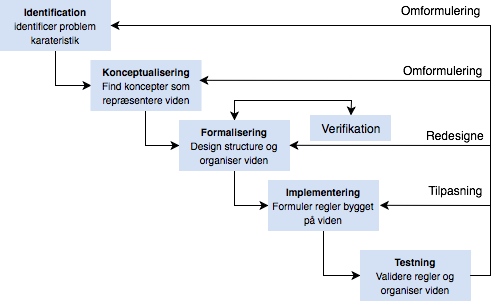
\includegraphics[width=1\textwidth]{Statusseminar/metode.png} 
%	\caption{XXXX.}
%	\label{fig:metode}  
%\end{figure}
%
%
%Da input-output relationen allerede er kendt anvendes supervised machine learning. Da formålet er at identificere hvilken kategori en ny observation tilhører anvendes klassificering.  

%
%\section{Data forberedelse} / Model
%- segmentation
%- farvetransformation - text/tal
%
%\section{Klassifikation}
%\subsection{Machine learning}
%\subsection{Feature for klassificering}
%\subsection{Neurale netværk som klassificering}
%
%\section{Validering}
%- klassificering performance matrics 
%
%
%dataindsamling
%data processering 
%feature extraction 
\chapter{Resultat}
\textit{I dette kapitel beskrives resultatet for evaluering af systemets anvendelighed i forhold til at besvare problemformuleringen. I denne forbindelse er systemets performans og brugbarhed evalueret.}

\section{Systemets performans}
*** TILFØJ DET MED RANGORDRE *** \\
Ud af 33 lægemidler var der 13 lægemidler, hvor der var enighed  mellem forsøgspersonerne. Der var enighed om at 11 lægemidler ikke krævede uddybende samt at 2 lægemidler krævede uddybende information ved implementering af disse i klinikken. Af 11 testpersoner vurderede 9 at størstedelen af lægemidlerne ikke krævede uddybende information, mens 2 testpersoner vurderede at størstedelen af lægemidlerne krævede uddybende information, hvilket er markeret med blåt i Tabel \ref{table:test1}. Gennemsnittet blev vurderet til at 12,27 lægemidler, svarende til 37,19~\%, krævede uddybende information, mens 20,63 lægemidler, svarende til 62,5~\%, ikke krævede uddybende information, hvilket ligeledes fremgår af Tabel \ref{table:test1}. 

\begin{table}[H]
\caption{Krydstabel for vurderingen ja eller nej i forhold til uddybende information om lægemiddelskiftet og testpersoner samt lægemiddel Nyt, som er indikeret som nummer 12. \textcolor{red}{Er i tvivl, hvorvidt det giver mening at have lægemiddel Nyt med i denne test}}
\vspace{2mm}
\label{table:test1}
\centering
\begin{tabular}{l|c|c|c|c|c|c|c|c|c|c|c|c|c}
\rowcolor[HTML]{C0C0C0}
 & \multicolumn{11}{|c|}{\textbf{Testperson}} & \textbf{} & \textbf{Total}    \\
\rowcolor[HTML]{C0C0C0}  & \textbf{1}  & \textbf{2}  & \textbf{3} & \textbf{4} & \textbf{5} & \textbf{6} & \textbf{7} & \textbf{8} & \textbf{9} & \textbf{10} & \textbf{11} & \textbf{12}  & \\ 
\cellcolor[HTML]{C0C0C0}{Antal af Nej}            & 24 & 20 & 21  &  28 &  15 &  21 & 17   &  12  & 21  & 26   &  22  & 29 & 256      \\ \cline{2-13}
\cellcolor[HTML]{C0C0C0}{\% af Nej }  & 9,4 & 7,8  & 8,2 & 10,9  & 5,9  &  8,2 & 6,6  & 4,7  & 8,2 & 10,2  &  8,6 & 11,3 &  100    \\ \cline{2-13}
\cellcolor[HTML]{C0C0C0}{\% af Gruppe} & 72,7 &  60,6  & 63,6 & 84,8   & 45,5   & 63,6  & 51,5  & 36,4 & 63,6 & 78,8 & 66,7  & 87,9 & 64,6 \\ \cline{2-13}
\cellcolor[HTML]{C0C0C0}{\% af Total}  & 6,1 & 5,1 & 5,3  & 7,1 & 3,8 & 5,3  & 4,3 & 3,0  & 5,3 & 6,6  & 5,6  & 7,3 &  64,6 \\ \hline
\cellcolor[HTML]{C0C0C0}{Antal af Ja} & 9 & 13 & 12 & 5  &  \cellcolor{blue}{18} & 12  & 16  &  \cellcolor{blue}{21}  & 12 & 7  & 11 & 4 & 140    \\ \cline{2-13} \cellcolor[HTML]{C0C0C0}{\% af Ja}  & 6,4 & 9,3  & 8,6 & 3,6 & 12,9  & 8,6  & 11,4 & 15  & 8,6  & 5,0 & 7,9  & 2,9 & 100   \\ \cline{2-13}
 \cellcolor[HTML]{C0C0C0}{\% af Gruppe} & 27,3 & 39,4 & 36,4 & 15,2   & 54,5  & 36,4 & 48,5 & 63,6  & 36,4 & 21,2 & 33,3  & 12,1 & 35,4      \\ \cline{2-13}
\cellcolor[HTML]{C0C0C0}{\% af Total}  & 2,3   & 3,3 & 3,0 & 1,3 & 4,5 & 3,0 & 4,0 & 5,3 & 3,0 & 1,8 &  2,8  & 1,0 &  35,4     \\ \hline  \cellcolor[HTML]{C0C0C0}{Total}  & 33 & 33 & 33  & 33  & 33  & 33  & 33  &  33 &  33 &   33 &  33  &  33 &  396     \\ \cline{2-13}
 \cellcolor[HTML]{C0C0C0}{\% af Nej og Ja}  & 8,3    & 8,3    &  8,3  & 8,3   &  8,3  &  8,3  &  8,3  &  8,3  & 8,3   & 8,3    & 8,3    &  8,3 &  100    \\ \cline{2-13}
 \cellcolor[HTML]{C0C0C0}{\% af Gruppe} & 100   & 100   &  100 &  100 &  100 &  100 &  100 & 100  & 100  & 100   &  100  & 100 &      100 \\ \cline{2-13}
\cellcolor[HTML]{C0C0C0}{\% af Total} & 8,3    & 8,3    &  8,3  & 8,3   &  8,3  &  8,3  &  8,3  &  8,3  & 8,3   & 8,3    & 8,3    &  8,3 &  100   \\
\end{tabular}
\end{table}

Test for sammenhængen mellem svarene ja eller nej i forhold til om der kræves uddybende information i forhold til lægemiddelskiftet fremgår af Tabel \ref{table:test2}.

\begin{table}[H]
\caption{Person chi-square test.}
\vspace{2mm}
\label{table:test2}
\centering
\begin{tabular}{l|p{2cm}|p{2cm}|p{4.5cm}}
\cellcolor[HTML]{C0C0C0}\textbf{} & \cellcolor[HTML]{C0C0C0}\textbf{Værdi} & \cellcolor[HTML]{C0C0C0}\textbf{df} & \cellcolor[HTML]{C0C0C0}\textbf{Asymptotisk Signifikant (2-siddet)} \\ \hline
\cellcolor[HTML]{C0C0C0}\textbf{Pearson Chi-Square} & 37,21 & 11 & 0,000 \\
\end{tabular}
\end{table}

Da P<0,001  vil dette sige at der er statistisk signifikant sammenhæng mellem om der er svaret ja eller nej og testpersonerne. Dette vil sige at der er forskel på hvordan testpersonerne har vurderet hvert enkelt lægemiddelskift.


\section{Systemets brugbarhed}
Systemet blev vurderet som et brugbart hjælpeværktøj i forhold til at oplysninger om lægemiddelskiftet kan genereres automatisk, hvormed der kan bruges mindre tid på helt simple skift. Dog skal systemet ikke overtage, da erfaringen inden for området stadig har stor betydning for vurderingen. 

Det blev vurderet at funktioner, såsom Look-a-like og Medicinrådet, ikke nødvendigvis skulle vægtes lige højt mellem funktioner, da det afhænger af den enkelte situation. Look-a-like vægtes generelt ikke særligt højt, hvoraf antallet af egenskaber der skifter er mere afgørende for kompleksiteten såsom f.eks. holdbarhed, emballage og konserveringsmidler. I forhold til Medicinrådet blev det vurderet at det ikke var vigtigt, hvorvidt lægemidlet indgik i Medicinrådets behandlingsvejledning, men om der var foretaget ændringer i denne var mere interessant og kunne have en betydning. 

I forhold til videreudvikling blev det vurderet at systemet skal have flere problemstillinger som input, såsom pris i forhold til hvor meget det koster og hvor meget der forbruges samt hvor mange patienter og afdelinger som anvender lægemidlet. Derudover bør granuleringen af look-a-like, navneændring og dispenseringsform i forhold til vægtningen af risikoscoren, da nogle ændringer vil kunne ligestilles og derfor ikke have betydning for klinikken. Der skal ligeledes skelnes mellem styrke og styrkeangivelse, da ændringerne ved styrkeangivelse ikke vil have en betydning, hvis pakningsstørrelsen ikke er ændret. Systemets anvendelighed blev derudover perspektiveret i forhold til at kunne anvendes til andre processer i forbindelse med lægemiddelskift såsom at anvende et lignende systemet inden udbuddet på lægemidler er fastlagt.




\subsection{Noter fra diskussion}

1: Look-a-like vægter de ikke højt – har de også fået at vide fra Amgros – klinikken er efterhånden vant til at LM skifter navne. Det afhænger af om der også er andre faktorer, som har en betydning.
Medicinrådet i sig selv er ikke nødvendigvis årsag til at det bliver kompliceret – eksempel Mabthera-skift – antallet af egenskaber der skifter er mest afgørende
Holdbarhed, emballage, konserveringsmiddel har også betydning for kompleksiteten. \\
2:Look-a-like – måske skal der flere bogstaver med – den kobler pt for nemt. 
Charlotte synes, at det kunne være rart, hvis disse oplysninger kunne komme af sig selv. Hun er begejstret for værktøjet.
Medicinservice vil altid have forbrugende afdelinger i tankerne, når de skal vurdere kompleksiteten i skiftet. Det kunne måske være en god ide at koble data på forbrug på.
Det kommer også an på prisen (Hvad koster det at skifte? Hvor meget forbruges? Hvor mange patienter?)
\\3:Janne synes, at det kunne være et fint hjælpeværktøj – kunne bruge mindre tid på helt simple skift – men man skal selvfølgelig ikke slå hjernen fra. Hvis der ikke er sket en ændring i Medicinrådets vejledninger, har det måske ikke den store betydning.  \\
4:Look-a-like giver ikke den store værdi.
Navneændring – det kan være svært fra skift til skift – kunne man gå mere i dybden med at graduere scoren afhængig af ex. skift fra original til generisk.
Dispenseringsform – her kunne man også differentiere/graduere scoren, fx er dispergible tabletter til frysetørrede tabletter betyder ikke noget for klinikken. \\
5:Det er et godt udgangspunkt. Kunne også godt anvendes inden udbuddet – gøre opmærksom på, hvor der er kritiske områder.
Hvis vi kan føde værktøjet med flere problemstillinger, vil det være rigtig godt.
Hvis de skifter styrkeangivelse, men ikke pakningsstørrelse, så har det ikke den store betydning.
Klinisk Farmakologisk Enhed (KFE) styrer skift i prioritering fra Medicinrådet (behandlingslinjeændring).

%% Afrunding %%


\chapter{Diskussion}
\textit{I dette kapitel diskuteres metode og resultater i forhold til at besvare problemformuleringen.}

%Hvorfor virker det anvendeligt for dem? Og hvorfor gør det ikke? Hvordan kan det videreudvikles i forhold til nu? Medarbejdernes erfaring er vigtigt

\section{Opsummering af resultater}
Flere lægemiddelskift er vurderet af medarbejderne til at skulle rangeres lavere end systemet. En tendens forekommer for lægemiddelskift, hvor risikofaktorer, såsom look-a-like, Medicinrådet og ATC-kritiske, indgår i risikoscoren. Systemets risikofaktorer og vægtningen af disse skal derfor overvejes i forhold til anvendeligheden. Ligeledes blev det belyst, at erfaringer har en stor indflydelse på risikovurderingen, hvormed det kan diskuteres, hvorvidt inkorporering af andre risikofaktorer kan forbedre systemets anvendelighed.

Systemets performance blev vurderet til at være god, med et areal under kurven på 0,840, i forhold til at forudsige hvornår et lægemiddelskift kræver uddybende information. På baggrund af dette er grænseværdier fastsat og ud fra dette er lægemiddelskift inddelt ud fra risikoscoren i forhold til, hvornår et lægemiddelskift kræver ingen opmærksomhed, begrænset opmærksomhed, opmærksomhed og særlig opmærksomhed. Systemets performance skal diskuteres i forhold til andre systemer. 

Da systemet blev anvendt til at undersøge anvendeligheden af et regelbaseret system til risikovurdering af lægemiddelskift, skal det overvejes, hvad der kræves for implementeringen af et endeligt system samt hvilken vedligeholdelse systemet kræver og hvilke udfordringer der kan være relateret til dette. 

\section{Risikofaktorer og vægtning}
Look-a-like vurderes ikke af medarbejderne i den nuværende vurdering og er derfor ikke vægtet høj ved risikovurderingen. Det kan derfor diskuteres, hvorvidt funktionen er anvendelig. I klinikken kan forvirring over lignende navn opstå og lede til medicineringsfejl, jævnfør Afsnit \ref{sec:ProblemLaeg}, hvorfor opmærksomhed på look-a-like er anvendeligt for klinikken. Look-a-like anses ikke for at være vigtig i risikovurderingen af lægemiddelskift og bør derfor ikke vægtes ved beregning af risikoscoren, men tilgængeligheden af denne i forhold til at informere klinikken om look-a-likes er stadig relevant.
Derudover kan koblingen af look-a-like med f.eks. dispenseringsform eller terapiområde gøre funktionen mere anvendelig ved at look-a-like ikke kun er defineret ud fra lægemidlets navn, men for lægemiddelnavne med samme dispenseringsform eller terapiområde. Ligeledes kan det overvejes, hvorvidt look-a-likes skal defineres af eksperter på området, hvormed sammenligningen mellem lægemiddelnavne er sat i relation og derfor vil det kunne forventes at være mere relevant og anvendelig.

Lægemiddelskift, som indgår i Medicinrådets behandlingsvejledning, blev vurderet til ikke at have en betydning medmindre, at der var foretaget ændringer i behandlingsvejledningen. Ligeledes blev det påvist, at antallet af ændringer i behandlingsvejledningen har betydning for kompleksiteten, hvormed det skal diskuteres, hvorvidt der skal differentieres mellem antallet af ændringer for at optimere anvendeligheden af risikofaktoren. Lægemidler, som indgår i Medicinrådets behandlingsvejledning anses derfor ikke som vigtig i risikovurderingen, hvormed denne ligeledes ikke bør vægtes ved beregningen af risikoscoren, men stadig være tilgængelighed for at gøre medarbejderne opmærksomhed på dette og derved vurdere, hvorvidt det har relevans for det enkelte lægemiddelskift.

Graden af differentiering inden for hver risikofaktorer skal vurderes i forhold til at opnå en bedre anvendelighed af systemet. Dette gælder både for ændringer i lægemidlets navn, f.eks. ved skift fra originalt til generisk, dispenseringsform og styrke. Ligeledes skal dispenseringsformer ligestilles, da f.eks. skift fra dispergible tabletter og frysetørrede tabletter, ikke har betydning for klinikken samt at ændringer i styrke kan variere alt efter om det er den reelle styrke eller styrkeangivelsen der er ændret. Dette vil kræve at tilfælde, hvor ændringer kan ligestilles identificeres samt at gradueringsgraden for hver risikofaktor defineres af én ekspert eller flere eksperter før det implementeres i systemet. Dertil skal det vurderes, hvorvidt nogle ændringer skal prioriteres højere end andre. 

\section{Inkorporering af risikofaktorer}
Risikovurdering af lægemiddelskift er meget erfaringsbaseret og flere faktorer vurderes af medarbejdere end der indgår i systemets risikovurdering såsom, hvilke afdelinger der anvender det, hvor mange patienter samt hvor meget lægemiddelskiftet koster. For at inkorporere dette i systemet, vil det kræve at systemet kobles med data om forbrug i forhold til afdelinger og historisk data om prisniveauer på medicin. Ligeledes kræves det at der defineres en grænse for, hvornår disse faktorer vil medvirke til at lægemiddelskiftet er kritisk. Dette kan være vanskeligt at definere, da det afhænger af mange faktorer som f.eks., hvilken afdeling der er involveret, hvorvidt denne afdeling har erfaring med lægemiddelskift og derfor er mere eller mindre opmærksom på ændringer. Dette skal ligeledes vurderes i forhold til, hvor meget lægemidlet koster ud fra hvor mange afdelinger og patientgrupper som anvender lægemidlet. Dertil skal det vurderes, hvorvidt risikofaktorer, som er erfaringsbaseret, skal inkorporeres i systemet eller om vurderingen af disse håndteres bedre af én ekspert eller flere eksperter inden for området.

\section{Systemets performance}
Ud fra sammenligningen med andre studier som foretager risikovurdering af diagnostiske tests performer systemet til risikovurdering af lægemiddelskift ligeværdigt~\citep{Chan2009,VanStraten2010}. For et multistudie, der undersøger performancen af systemer til forudsigelse af risikoen for kardiovaskulære sygdomme for patienter med diabetes, varierede arealet under kurven mellem 0,64 og 0,49~\citep{Chan2009}, hvilket henholdsvis indikerer en mindre nøjagtig og en ikke informativ test~\citep{Greiner2000}. Dette vil sige, at systemet til risikovurderingen af lægemiddelskift preformer bedre, med et areal under kurven på 0,84. Modsat er det i et andet multistudie, som undersøger performance af systemer til risikovurdering af patienter som får foretaget en koronararterie bypass, påvist et areal under kurven på over 0,80 for begge systemer~\citep{VanStraten2010}, hvilket er ligeværdigt med systemet til risikovurdering af lægemiddelskift.

Det kan diskuteres, hvorvidt studierne er sammenlignelige med systemet til risikovurdering af lægemiddelskift, da antallet af samples i studierne er 
højere og derved kan medvirke til en større variation i systemernes performance. Derudover er der anvendt forskellige metoder til vægtningen af risikofaktorerne, hvilket ligeledes kan have en indflydelse. Samtidig er risikovurderingen foretaget ud fra risikofaktorer, som er kendetegnet ved patienten, hvormed der kan være mange uforudsete faktorer, som kan influere i forhold til systemets output og derved afspejles af systemets performance. 

\section{Implementering og vedligeholdelse}
Implementering af systemet vil kræve at der bestemmes, hvilke risikofaktorer der skal anvendes samt hvordan vægtningen og gradueringen af disse fastsættes. Denne proces kan varetages ved inputs fra eksperter på området for at opnå en fælles konsensus. Derudover skal det undersøges, hvordan opmærksomheden på lægemiddelskiftene skal visualiseres for brugervenligheden ved f.eks. farveindikationer eller ved en bestemt rangorden. 

Det vil ligeledes kræve en optimering af præprocessering af data eller at data fremadrettet bliver indsamlet struktureret for at systemet kan tage højde for variationen i data, som f.eks. forkortelser ved dispenseringsform. Det kan diskuteres, hvorvidt det er muligt at indsamle data struktureret, da det ikke er SRN som står for dette. Derudover kan det overvejes om Levenshtein Distancen kan anvendes til sammenligning af ord, hvormed mindre variationer i data kan tillades. Dette kan f.eks. gøre ved at definere et antal af operationer som må være forskellige ved sammenligning.

Samtidig kræver det, at der udarbejdes en brugergrænseflade for medarbejderne før anvendelse af systemet, hvilket skal give medarbejderne mulighed for at indlæse et skifteliste for et nyt år, for derefter at gemme skiftelisten med systemets output. Derudover vil det kræve at brugeren af systemet, herunder medarbejderne fra SRN, har kendskab til system og kan se fordelene ved at anvende systemet. Samtidig skal der ved implementering af systemet tages højde for forandringer i risikovurdering af lægemiddelskift. Da systemet er et regelbaseret system kan justeringer foretages uden at dette påvirker andre dele af systemet. Dette kan imidlertid medvirke til, at systemet bliver for kompleks, hvormed det skal vurderes, hvorvidt andre metoder, som f.eks. statistiske metoder er mere hensigtsmæssige at benytte.


%Overensstemmelsen mellem systemet og medarbejdernes vurdering af lægemiddelskift er begrænset. Systemet har en højere specificitet end sensitivitet, hvilket betyder, at systemet er bedre til at identificere lægemiddelskift, som ikke kræver uddybende information sammenlignet med lægemiddelskift, som kræver uddybende information. Ligeledes har systemet en høj type 2 fejl, hvilket betyder, at systemet vurderer lægemiddelskift, hvor der kræves uddybende information til ikke at kræve uddybende information. 

%I forhold til risikoscoren blev det påvist, at medarbejdernes vurdering var mere nøjagtig sammenlignet med systemet, hvilket vil sige at medarbejderne vurdering har en højere sensitivitet og lavere specificitet end systemet. \textcolor{red}{skriv til her i forhold til diskriminationsgrænse.}

%Systemets er vurderet af medarbejdere fra SRN til at være et godt udgangspunkt for et hjælpeværktøj i forbindelse med risikovurdering af lægemiddelskift, men at risikofaktorerne og vægtningen af disse skal granuleres i forhold til at forbedre risikoscoren. Derudover blev funktioner såsom look-a-like og Medicinrådet vurderet til ikke at blive vægtet særligt højt ved lægemiddelskiftet, men at det i kombination med antallet af ændrede faktorer kunne have en betydning for lægemiddelskiftet.

%\section{Risikovurdering}
%Risikovurderingen afspejler ikke den nuværende vurdering af lægemiddelskift, hvilket kan skyldes, at der var variation mellem medarbejderne vurdering af lægemiddelskift. Dette kan være på grund af, at medarbejderne var repræsenteret fra forskellige afdelinger og derved havde forskellige vurderinger af lægemiddelskiftene set ud fra den afdeling de repræsenterede. Samtidig kan medarbejdernes vurdering være præget af erfaringer som systemet ikke tager højde for i vurderingen, hvilket kan medvirke til, at nogle lægemidler er vurderet til ikke at kræve uddybende information af medarbejderne men at systemet vurderer dette. Dette understøttes af en medarbejder, hvis generelle  kommentar var, at det var svært ikke at tage deres erfaring med i vurderingen, hvilket fremgår af Tabel \ref{table:resultat2} i Appendiks \ref{App:Resultat}. Til trods for, at dette blev gjort opmærksom på via introduktionen, der blev givet inden risikovurderingen, som fremgår af Appendiks \ref{App:Intro}. Derudover kan der være andre ændrede faktorer som skyldes, at lægemiddelskiftet, er uddybet af Lægemiddel Nyt, såsom ændret form, størrelse og farve på lægemidlet, hvilket er beskrevet i Afsnit \ref{sec:ProblemLaeg}, eller f.eks. ændring af pakningsstørrelse, som der i nogle tilfælde er uddybende kommentarer om i Lægemiddel Nyt, hvilket fremgår af Tabel \ref{table:Proces} i Afsnit \ref{sec:ImpLaeg}. I kraft af, at systemet ikke tager højde for disse ændringer kan det medvirke til, at nogle lægemiddelskift er uddybet af  Lægemiddel Nyt, men at disse ikke er vurderet af medarbejderne til at skulle uddybes, da deres vurderingen udelukkende er baseret på systemets output, herunder risikoscore og begrundelse for denne.
%
%\section{Risikoscore}
%%0-5~\%
%Medarbejderne kommenterede, at systemet i flere tilfælde vurderede et lægemiddelskift risikoscore for højt og derved skulle rangeres lavere. Dette kan skyldes, at medarbejdernes erfaring er medtaget i vurderingen i forhold til at kende skiftet og derved vil rangere dette lavere, hvilket understøttes af en medarbejder i kommentaren som fremgår af Tabel \ref{table:resultat2} i Appendiks \ref{App:Resultat}. Ligeledes blev det af flere medarbejdere pointeret at funktionerne look-a-like og Medicinråd var vægtet for højt. Årsagen til dette kan være, at  risikofaktorerne ikke tages med i den nuværende vurderingen, hvormed disse ikke prioriteres særligt højt.
%
%Systemet skelner ikke i forhold til om der er ændring i styrken eller  styrkeangivelsen, hvormed et lægemiddelskift med samme risikoscore kan være vurderet forskelligt ud fra, hvorvidt lægemiddelskiftet kræver uddybende information. Dette understøttes af kommentarer om tvivl i forhold til styrke fra flere medarbejdere, jævnfør Tabel \ref{table:resultat2} i Appendiks \ref{App:Resultat}. Dette vil kræve, at systemet ved sammenligning af ændring i styrke kombineres med, hvorvidt der er sket ændringer i pakningsstørrelse.\textcolor{red}{Tilføj i forhold til diskriminationsgrænse.}
%
%\section{Risikofaktorer og deres vægtning}
%Risikofaktorer, som look-a-like, blev vurderet af medarbejderne til ikke at have den store betydning for lægemiddelskift, hvormed vægtning af denne er for høj. Dette kan skyldes, at look-a-like funktion, udelukkende kigger i forhold til sammenligning af lægemidlets navn og ikke tager højde for om andre faktorer som, f.eks. dispenseringsform eller tepariområde, er ens for de lægemidler som er hinandens look-a-like. Derudover kan det være at look-a-like skal vægtes lavere eller udelades fra risikovurderingen, men stadig være tilgængelige i klinikken i forhold til at mindske fejlmedicinering opstået ved forvirring over sammenlignelige lægemiddelnavne, jævnfør Afsnit \ref{sec:ProblemLaeg}.
%
%Ligeledes blev Medicinrådet vurderet til ikke at skulle vægtes høj, da det at et lægemiddel indgår i behandlingsvejledningen i sig selv ikke har betydning, men at ændringer af faktorer og hvor mange der ændres har betydning. Dette kan skyldes, at Medicinrådet har en stor betydning første gang det implementeres i klinikken i forhold til at opnå besparelser eller hvis der sker ændringer, som kan forårsage fejlmedicinering, hvor betydningen efterfølgende er begrænset, hvorfor det er nødvendigt at systemet differentiere mellem dette.
%
%Det blev for navn, dispenseringsform og styrke vurderet af medarbejderne, at der ligeledes krævede granulering af ændringer i disse i forhold til vægtningen, da der var variationer i sværhedsgraden inden for hvert type af skift. Dette skyldes, at nogle skift anses som værende ligeværdige som f.eks. dispenseringsformer, der anvendes på samme måde i klinikken er af mindre betydning, sammenlignet med dispenseringsformer, som anvendes forskelligt i klinikken og derved har større betydning, hvis denne er ændret ved lægemiddelskift. Dette kræver, at der foretages en mere detaljeret præprocessering af data for at identificere ligeværdige typer af skift og samtidig have en større granuleringsgrad inden for hvert skift i forhold til vægtning af risikofaktorerne.

\chapter{Konklusion}
\textit{I dette kapitel konkluderes der på rapporten problemformulering i forhold til, hvorvidt et regelbaseret system er anvendeligt til risikovurdering af lægemiddelskift med henblik på at forbedre den nuværende vurdering af lægemiddelskift.}

Et regelbaseret system til risikovurdering af lægemiddelskift er anvendeligt i forhold til at forudsige, hvornår et lægemiddelskift kræver uddybende information. Derudover er det påvist, at risikocoren kan anvendes til at inddele lægemiddelskift ud fra hvor meget opmærksomhed de kræver, hvilket medvirker til at effektivisere den nuværende vurdering af lægemiddelskift.
Alligevel afspejler risikovurderingen på nogle områder ikke den nuværende vurdering af lægemiddelskift, hvormed systemet kræver yderligere tilpasning.

Det formodes, at ved tilpasning af systemet, at lægemiddelskift kan risikovurderes på samme vilkår som den nuværende vurdering og derfor vil være anvendeligt i risikovurdering af lægemiddelskift. Dertil, skal systemet stadig tiltænkes som et hjælpeværktøj, hvormed medarbejdernes erfaring skal tages med i den endelige vurderingen. 

På baggrund af dette skal yderligere studier undersøge, hvordan risikofaktorer skal granuleres og vægtes for at optimere anvendeligheden af systemet og derved forbedre den nuværende vurdering af lægemiddelskift.

\chapter{Konklusion}
\textit{I dette kapitel ....}


%%%% Kilder %%%%

\begingroup
	\raggedright
	\bibliography{bibtex/Maria}							% Litteraturlisten inkluderes
\endgroup


%%%% Fixme-listen %%%%

\newpage														% Ny side til Fixme-listen
\listoffixmes													% Fixme-listen - fjernes til sidst i projektet med "%"


%%%% Appendiks %%%%

\appendix
\chapter{Appendiks} \label{cha:AppA}
\section{Vurdering af lægemiddel}
Forinden et lægemiddel kan anvendes som standardbehandling foretager Medicinrådet og Amgros forskellige vurderinger af lægemidlet, hvilket er illustreret på figur \ref{fig:Udbud}.
 
\begin{figure}[H]\centering
	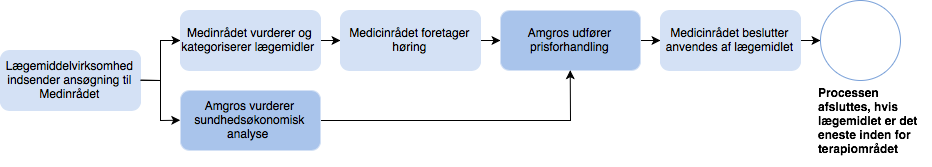
\includegraphics[width=1\textwidth]{billeder/Udbud.png} 
	\caption{Proces for vurdering af nye lægemidler.~\citep{DanskeRegioner2016}}
	\label{fig:Udbud}  
\end{figure}

Lægemiddelvirksomheder indsender som det første kliniske studier og sundhedsøkonomiske analyser til Medicinrådet med henblik på at ansøge om anvendelse af et nyt lægemiddel som standardbehandling~\citep{DanskeRegioner2016}. 

Efterfølgende kategoriserer Medicinrådet lægemidlet i merværdi på baggrund af ansøgningen samt en lægefaglig og statistisk vurdering.  Kategoriseringen inddeles i seks kategorier ud fra nuværende standardbehandling til stor, vigtig, lille, ingen, negativ og ikke-dokumenterbar merværdi~\citep{DanskeRegioner2016}. Yderligere høres Medicinrådets fagudvalg med henblik på at denne vurdering kan indgå i den samlede beslutning.~\citep{DanskeRegioner2016}

Parallelt med kategoriseringen forbereder Amgros en sundhedsøkonomisk analyse~\citep{DanskeRegioner2016} baseret på  samfundsomkostninger per patient for den nuværende og ansøgte behandling og samlede økonomiske konsekvenser for regionerne ved at anvende den ansøgende behandling ~\citep{Amgros2017, Amgros2017}. På baggrund af dette beregnes et prisinterval der danner grundlag for prisforhandlingen med lægemiddelvirksomhederne~\citep{DanskeRegioner2016}. 

Hvis den forhandlede pris er højere end den fastsatte kan lægemidlet ikke anbefales af Medicinrådet som standardbehandling~\citep{DanskeRegioner2016}. 
Er den forhandlede pris modsat lavere eller lig det fastsatte prisinterval og opfylder Medicinrådets faglige kriterier fremsendes en anbefaling til regionerne om anvendelse af lægemidlet som standardbehandling eller protokolleret anvendelse.
Ved protokolleret anvendelse tages lægemidlet i brug indtil der er tilstrækkeligt data til at Medicinrådet kan vurdere at lægemidlet kan anvendes som en fast behandling.~\citep{DanskeRegioner2016}

\section{Vurdering af ligeværdige lægemidler}
Hvis der er flere eksisterende lægemidler inden for samme terapiområde gennemgår lægemidlerne endnu en proces som fremgår af figur \ref{fig:Udbud1}. I denne proces har Medicinrådet til formål at udarbejde et national konsensus om anvendelse af lægemidlet inden for terapiområder~\citep{DanskeRegioner2016}. Processen varetages af fagudvalget, bestående af landets førende læger, der udarbejder forslag til fælles regionale behandlingsvejledninger. Disse forslag til behandlingsvejledningerne godkendes af Medicinrådet.~\citep{DanskeRegioner2016}

\begin{figure}[H]\centering
	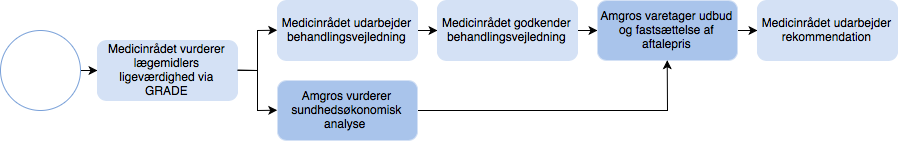
\includegraphics[width=1\textwidth]{billeder/Udbud1.png} 
	\caption{Proces for vurdering af ligeværdige lægemidler.~\citep{DanskeRegioner2016}}
	\label{fig:Udbud1}  
\end{figure}

Parallelt med udarbejdelse af forslag til behandlingsvejledning vurderer Amgros en sundhedsøkonomisk analyse~\citep{DanskeRegioner2016}. Amgros varetager herefter et udbud på baggrund godkendte  behandlingsvejledninger, hvorefter aftalepriser kan fastsættes og indføres i den sundhedsøkonomiske analyse.~\citep{DanskeRegioner2016}

Medicinrådet udarbejder til sidst en rekommandation, som omfatter det billigste lægemiddel, ud fra den behandlingsvejledningen fra fagudvalget og den sundhedsøkonomiske analyse~\citep{DanskeRegioner2016}. Rekommandationen indskrives herefter i behandlingsvejledningen og sendes til regionerne, der er ansvarlige for implementeringen af denne.~\citep{DanskeRegioner2016}

\chapter{Appendiks} \label{cha:AppB}
\section{Udbudstyper ved Amgrosudbud}
Udbudstyper er defineret på forhånd, enten på baggrund af lægemidlets pris, hvilket er tilfældet for de fleste lægemidler, eller ved økonomisk mest fordelagtige udbud, hvor prisen vægtes mod andre kriterier~\citep{Amgros2018a}. Disse kriterier er opstillet på baggrund af juridiske grundlag og kan f.eks. omfatte emballage, håndtering af lægemidlet ved administration samt patientsikkerhedsmæssige aspekter. Der kan være én eller flere vindere, hvilket medfører til fire typer af udbudsformer, hvilket fremgår af figur \ref{fig:TypeUdbud}.~\citep{Amgros2018a}

\begin{figure}[H]\centering
	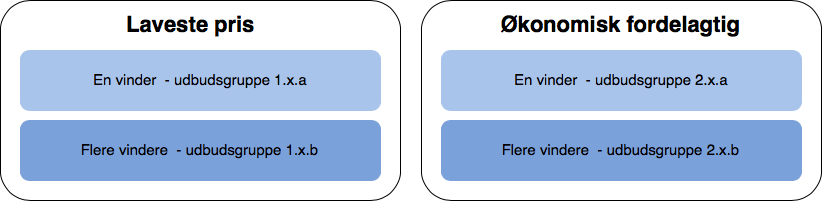
\includegraphics[width=0.7\textwidth]{billeder/TypeUdbud.png} 
	\caption{Udbudstyper inddelt i laveste pris og økonomisk fordelagtig. Tallene 1 og 2 angiver om der er én eller flere vindere, hvor bogstaverne a og b angiver én rammeaftale eller flere parallelle rammeaftaler. ~\citep{Amgros2018a}}
	\label{fig:TypeUdbud}  
\end{figure}

Hvis der er udbud af samme ATC-kode i flere udbudsgrupper vurderes det på baggrund af ATC-kodens årlige omsætning, hvorvidt lægemidlet  skal udbydes som et EU-udbud eller bagatelaftale(BA). EU-udbud sker hvis Apotekets Indkøbspris (AIP) er over 500.0000 kr. årligt og BA sker ved AIP under 500.000 kr. årligt. 

%*** SKAL OMSKRIVES \\
%Et EU-udbud af en ATC-kode dækker samtlige identikationer, hvilket betyder at tilbudsprisen vil være den samme for et lægemiddel uanset hvilken indikation det ordineres til, dette kan betyde at forskellige dispensionsformer og styrker af en given ATC-kode kan være udbudt i forskellige udbudsgrupper. 
%****
%
%\section{Typer af lægemiddelskift}
%Lægemiddelskift kan forekomme i forbindelse med kontraktskift, bagatelkøb eller restordre~\citep{Amgros2015}. Kontraktskift kan forekomme ved at lægemidlerne sendes i udbud, såkaldt amgrosudbud. Udbuddene forekommer hvis der findes mere end én leverandør af lægemidlet. Lægemidlerne bringes derved i konkurrence, hvilket kan give anledning til kontraktskift. I tilfælde af patent på lægemidlet, hvormed der kun findes én leverandør, er der ofte ikke konkurrence, da prisen på lægemidlet allerede er fastsat.~\citep{Amgros2015} 
%
%En gang årligt omkring maj eller juni publiceres bagatelkøb af Amgros, hvilket kan forårsage lægemiddelskift~\citep{Amgros2018}. I disse tilfælde modtager Amgros pristilbud fra leverandørere med henblik på økonomiske besparelser på lægemiddlerne~\citep{Amgros2012}. I disse tilfælde er Sygehusapoteket er ikke forpligtet til at anvende lægemidlet og leverandøren omfattes ikke af indkøbs- eller forsyningspligt, som ved kontraktskift.~\citep{Amgros2018}
%
%Restordre forekommer når efterspørgslen på et lægemiddel overstiger den tilgængelige mængde.~\citep{Amgros2015}. Dette kan f.eks. ske ved leveringesvigt fra leverandøren eller producenten på det ønskede lægemiddel~\citep{Amgros2017, Laegemiddelinformaion2017}. Leveringesvigt skyldes som ofte at producenten har mangel på råvarer eller produktionsvanskeligheder~\citep{Amgros2017, Laegemiddelinformaion2017}. I tilfælde  af restordre er det leverandørens ansvar at dække hospitalsapotekernes udgift ved indkøb af et erstatningslægemiddel\fxnote{KILDE}.
\chapter{Appendiks} \label{cha:AppC} 
\section{Indkøb af lægemidler}
Indkøb af lægemidler til distribution til de nordjyske hospitaler foretages af Sygehusapoteket Region Nordjylland (SRN)~\citep{SygehusapoteketRegionNordjylland2013}. Salg til Region Nordjyllands (RN) egne institutioner udgør 98,4~\% af det samlede salg i år 2012, hvor under 1~\% går til andre regioners sygehusapoteker og til private apoteker samt andre kunder. Udover indkøb yder SRN information og tilbyder tjenesteydelser til de kliniske afsnit, herunder klinisk farmaci.~\citep{SygehusapoteketRegionNordjylland2013}

Størstedelen af medicinindkøb i år 2012, svarende til 95~\%, skete via. Amgros. Yderligere blev 2~\% købt af andre sygehusapoteker, 1~\% fra private apoteker og 2~\% fra øvrige. ~\citep{SygehusapoteketRegionNordjylland2013}
Bestilling af medicin fra hospitalsafsnittene sker via medicinservice varetaget af farmakonomer. Der bestilles medicin via ApoVision-Online. SRN forgår som lagerholder og fremtager medicin manuelt fra henholdsvis almindeligt hyldelager, pater Noster (halvautomatik lager-reol) og høj-lager (paller).~\citep{SygehusapoteketRegionNordjylland2013}

SRN er opdelt i forskellige afdelinger herunder ledelse, administration, lægemiddelinformation, klinisk farmaci, logistik, kvalitetsafdeling og produktion. De primære aktører ved Amgrosudbud i RN er Amgros-ansvalige, Specialistfarmaceut/ATC-asnarlige og Lægemiddelinformation. Opgaver for disse aktører fremgår af figur\ref{fig:SRNudbud}.

\begin{figure}[H]\centering
	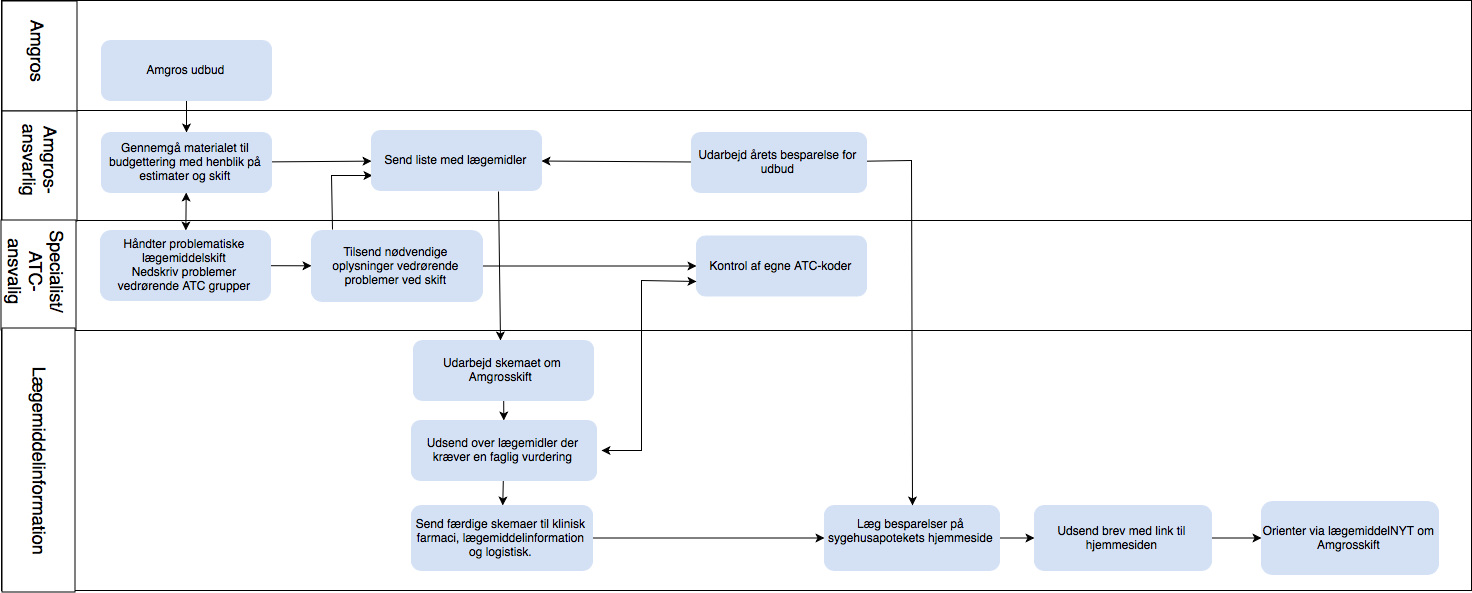
\includegraphics[width=1\textwidth]{billeder/SRNudbud.png} 
	\caption{...}
	\label{fig:SRNudbud}  
\end{figure}

Ved Amgrosudbud står den Amgros-ansvalige  for at gennemgå udbudsmaterialet og budgettestimere i forbindelse med kommende kontrakter. I sammenhæng med dette håndteres problematiske lægemiddelskift af specialist/ATC-ansvarlige. De problemer der vedrører ATC-grupper nedskrives og sendes tilbage til den Amgros-ansvarlige. Den Amgros-ansvarlige sender herefter en liste ud med lægemidler til Lægemiddelinformation, hvorefter der udarbejdes et skema om lægemiddelskift. Lægemiddelinformation udsender herefter en liste med lægemidler der kræver en faglig vurdering til Specialistfarmaceut/ATC-asnarlige, som kontrollere egne ATC-koder. Herefter sendes færdige skemaer til Klinisk farmaci, Lægemiddelinformationen og Logistik i SRN. Dernæst udarbejdes årets samlede besparelse af Amgros-ansvarlige og ligges på Sygehusapotekets hjemmeside af Lægemiddelinformationen som også sender brev med link til hjemmesiden og orientere via LægemiddelNyt omkring Amgrosskift. 
\chapter{Appendiks} \label{cha:AppD}
\textit{Dette appendiks indeholder forskellige instruktioner som Sygehusapoteket Region Nordjylland anvender i forbindelse med Amgrosskift. Det forekommer i følgende rækkefølge:}

\begin{enumerate}
\item Implementering af lægemiddelskift - skabelon til vurdering. 
\\Angivet i Appendiks på side \ref{XXX} og i litteraturlisten som~\citep{Sygehusapoteket2017}.  \label{item:ATC-ansvarlig}
%\item Amgrosudbud - Estimering af lægemiddelforbrug og opfølgning. Angivet i litteraturlisten som~\citep{Sygehusapoteket2017a}
%\item Implementering af lægemiddelskift. Angivet i litteraturlisten som~\citep{Sygehusapoteket2017b}
%\item Risikolægemidler lægemidler. \label{item:Risikolaegemidler} Angivet i litteraturlisten som [XX]
\item Skiftelister. Angivet i litteraturlisten som [XX] \label{item:Skiftelister}
\item Lægemiddel Nyt - Amgrosudbud og lægemiddelskift \label{item:Laegemiddelnyt}. Angivet i litteraturlisten som [XX] 
\end{enumerate}




%\includepdf[scale=0.8,pages=2-15,pagecommand={}]{mypages}
%\includepdf[scale=0.8,pages=16,pagecommand={}\label{appendix:bslut}]{mypages}
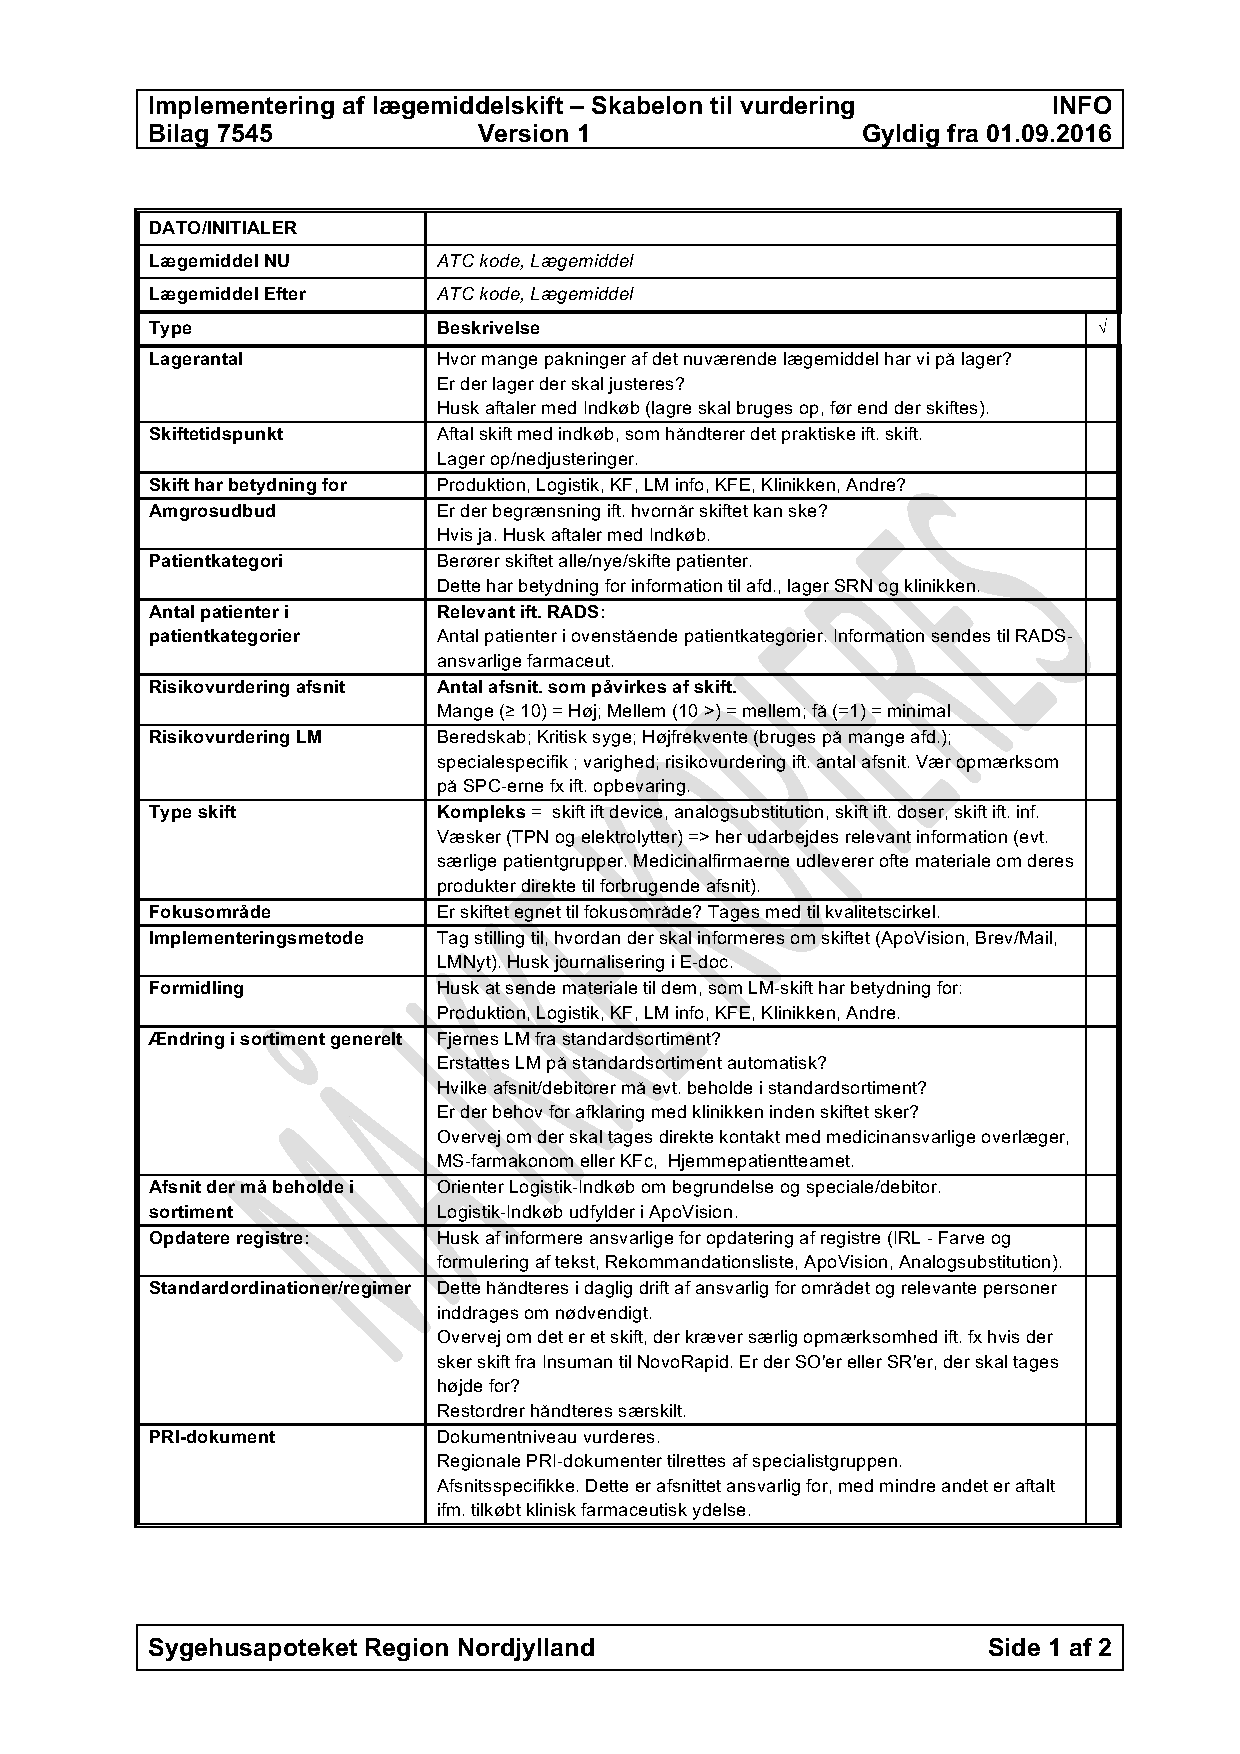
\includepdf[pages=1]{appendiks/Skabelon.pdf} 
%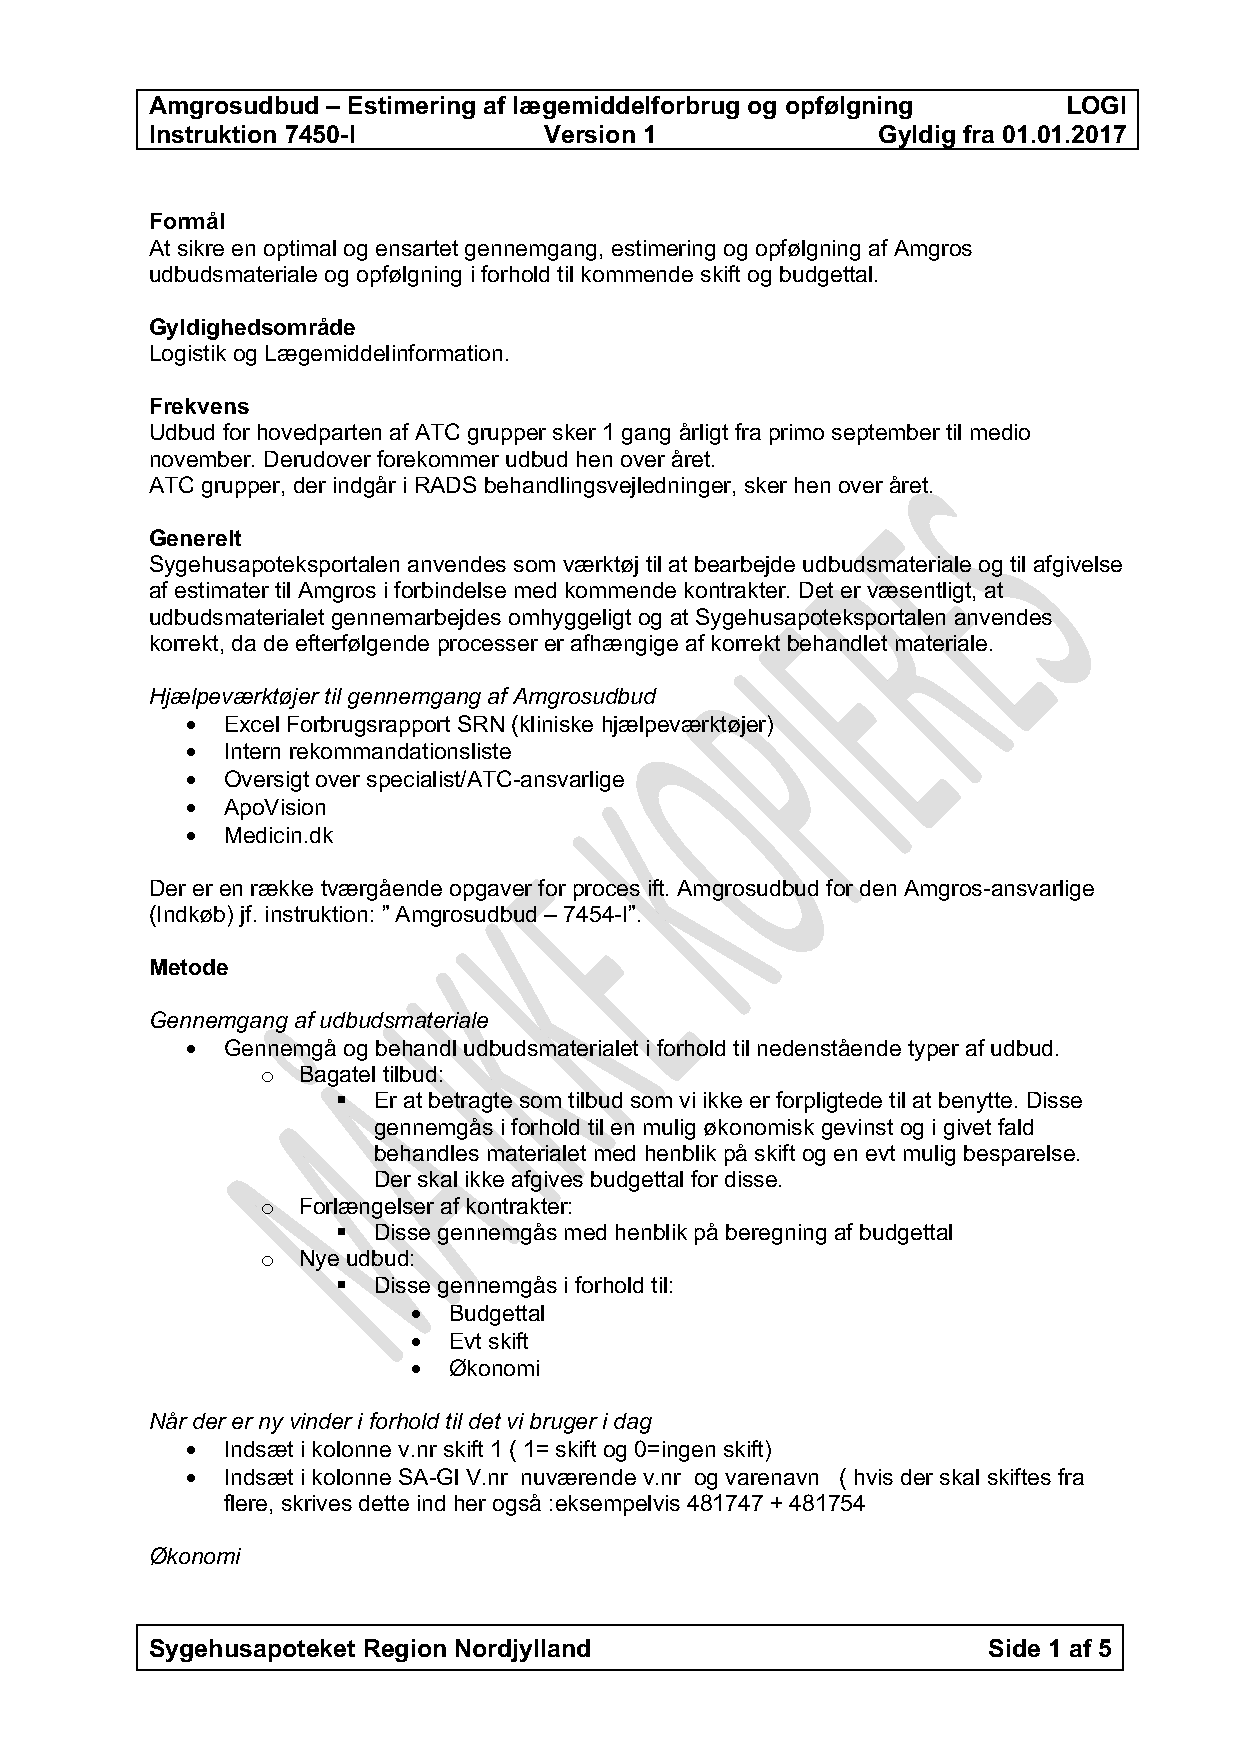
\includepdf[pages=1-3]{appendiks/Estimering.pdf}
%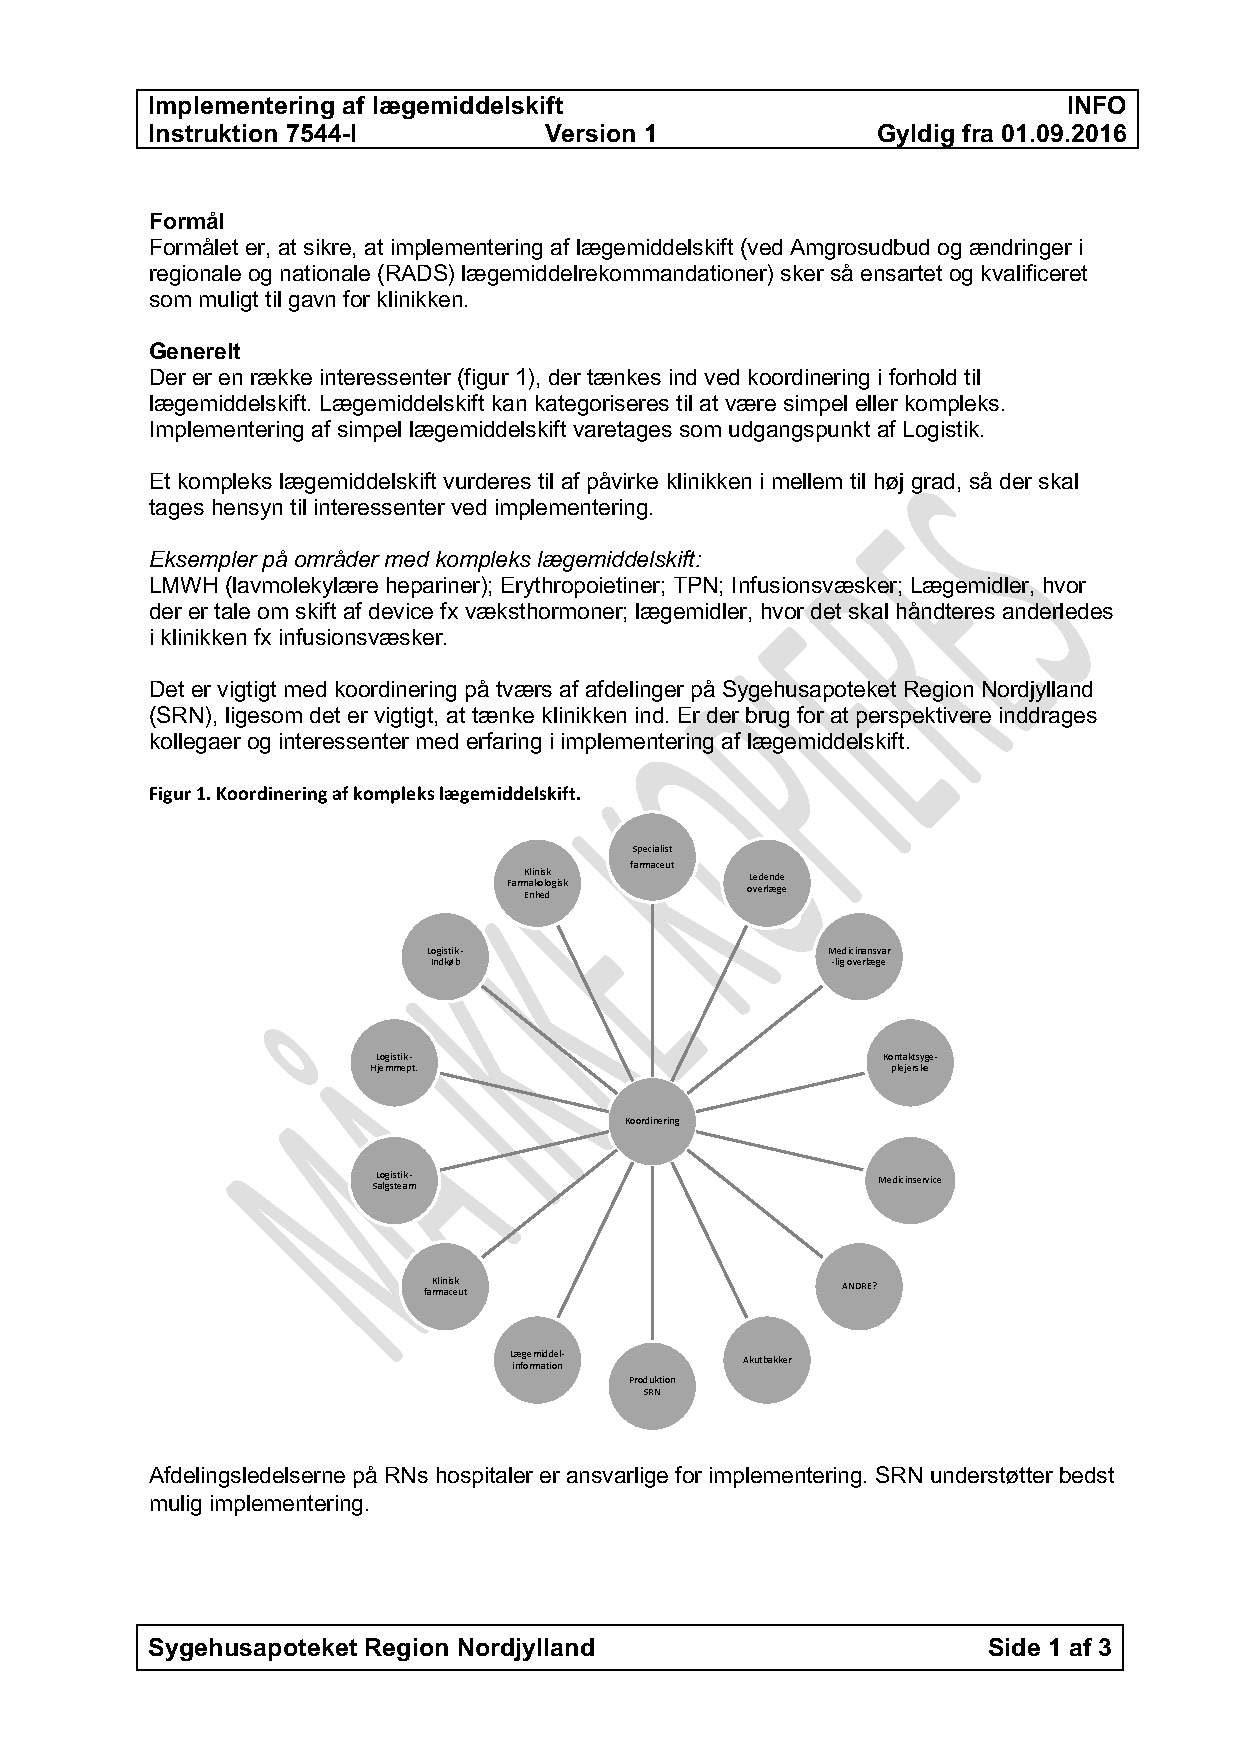
\includepdf[pages=1-2]{appendiks/Instruktion.pdf}
%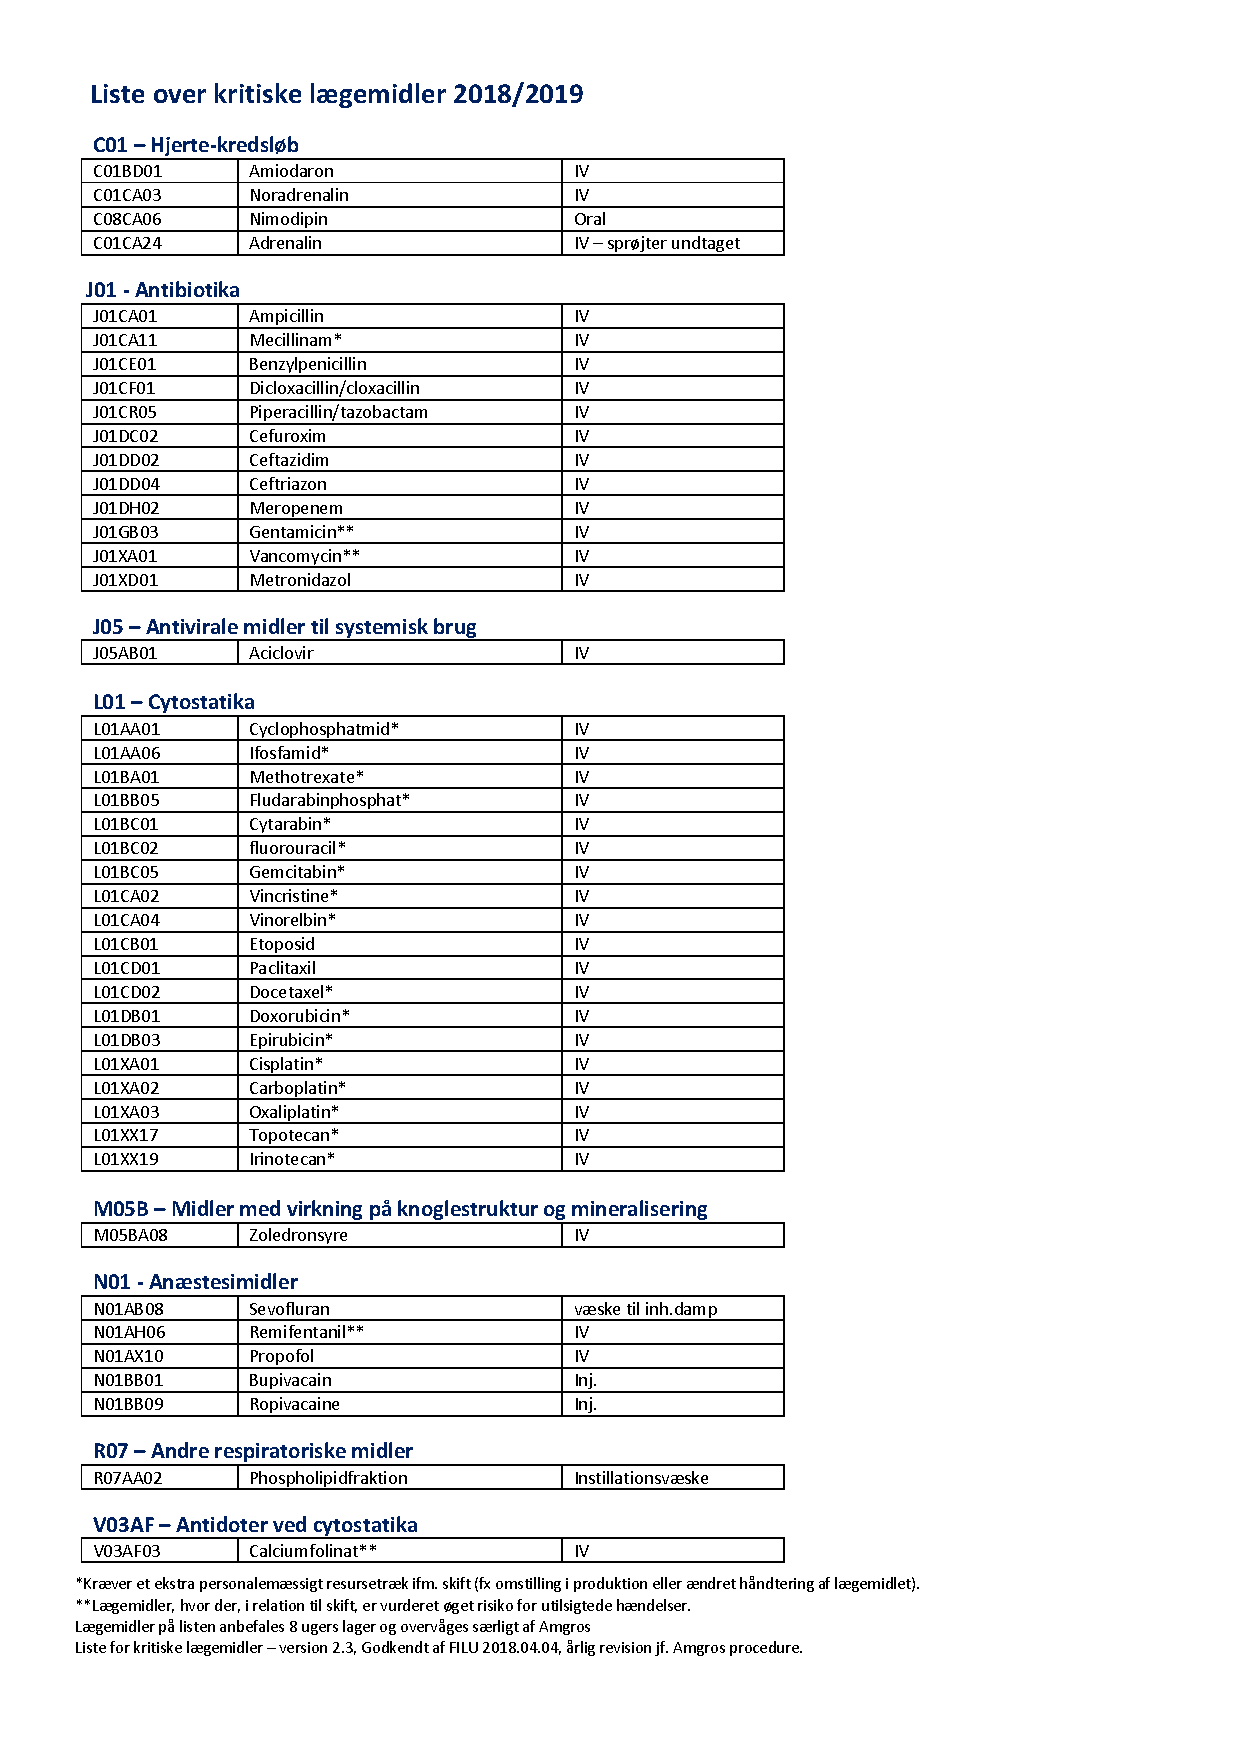
\includepdf[pages=1]{appendiks/Kistisklaegemidler.pdf}
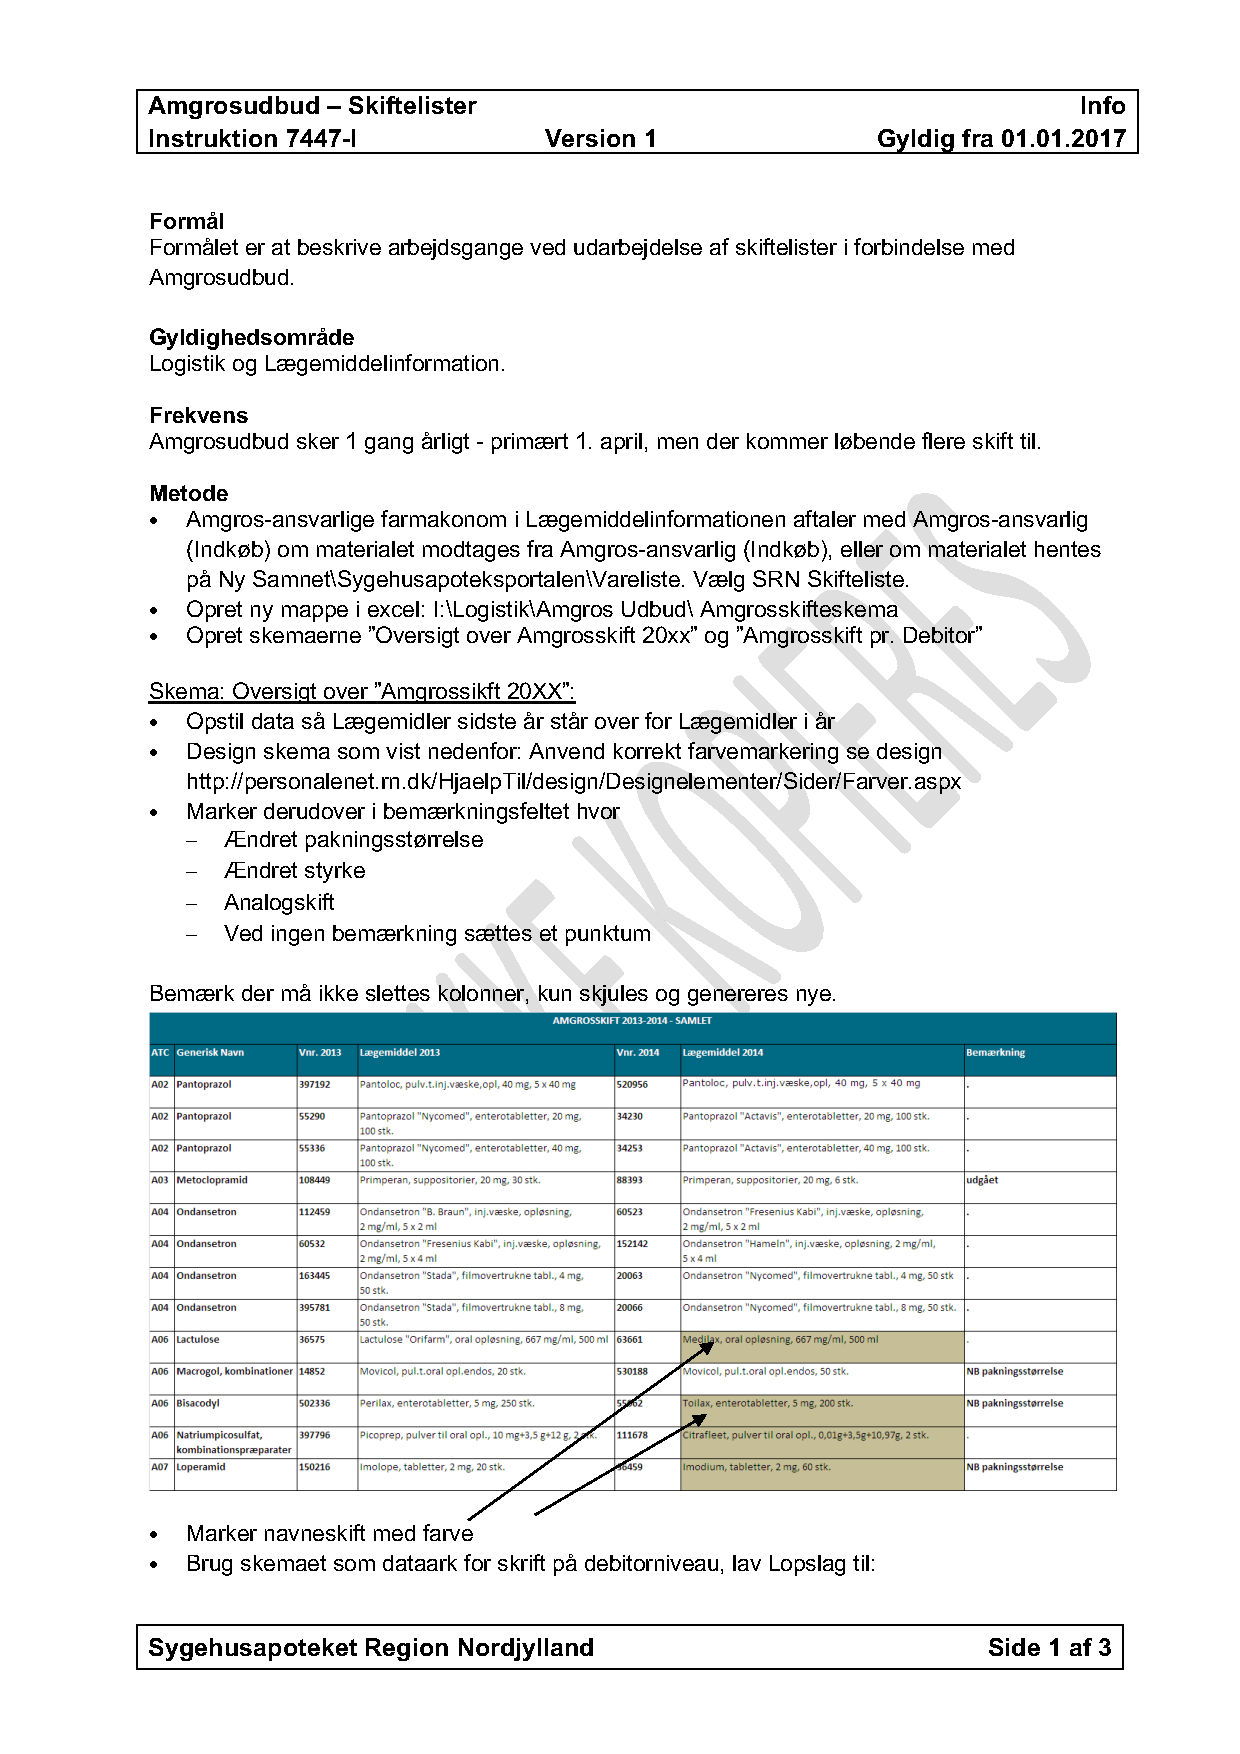
\includepdf[pages=1-3]{appendiks/Skiftelister.pdf}
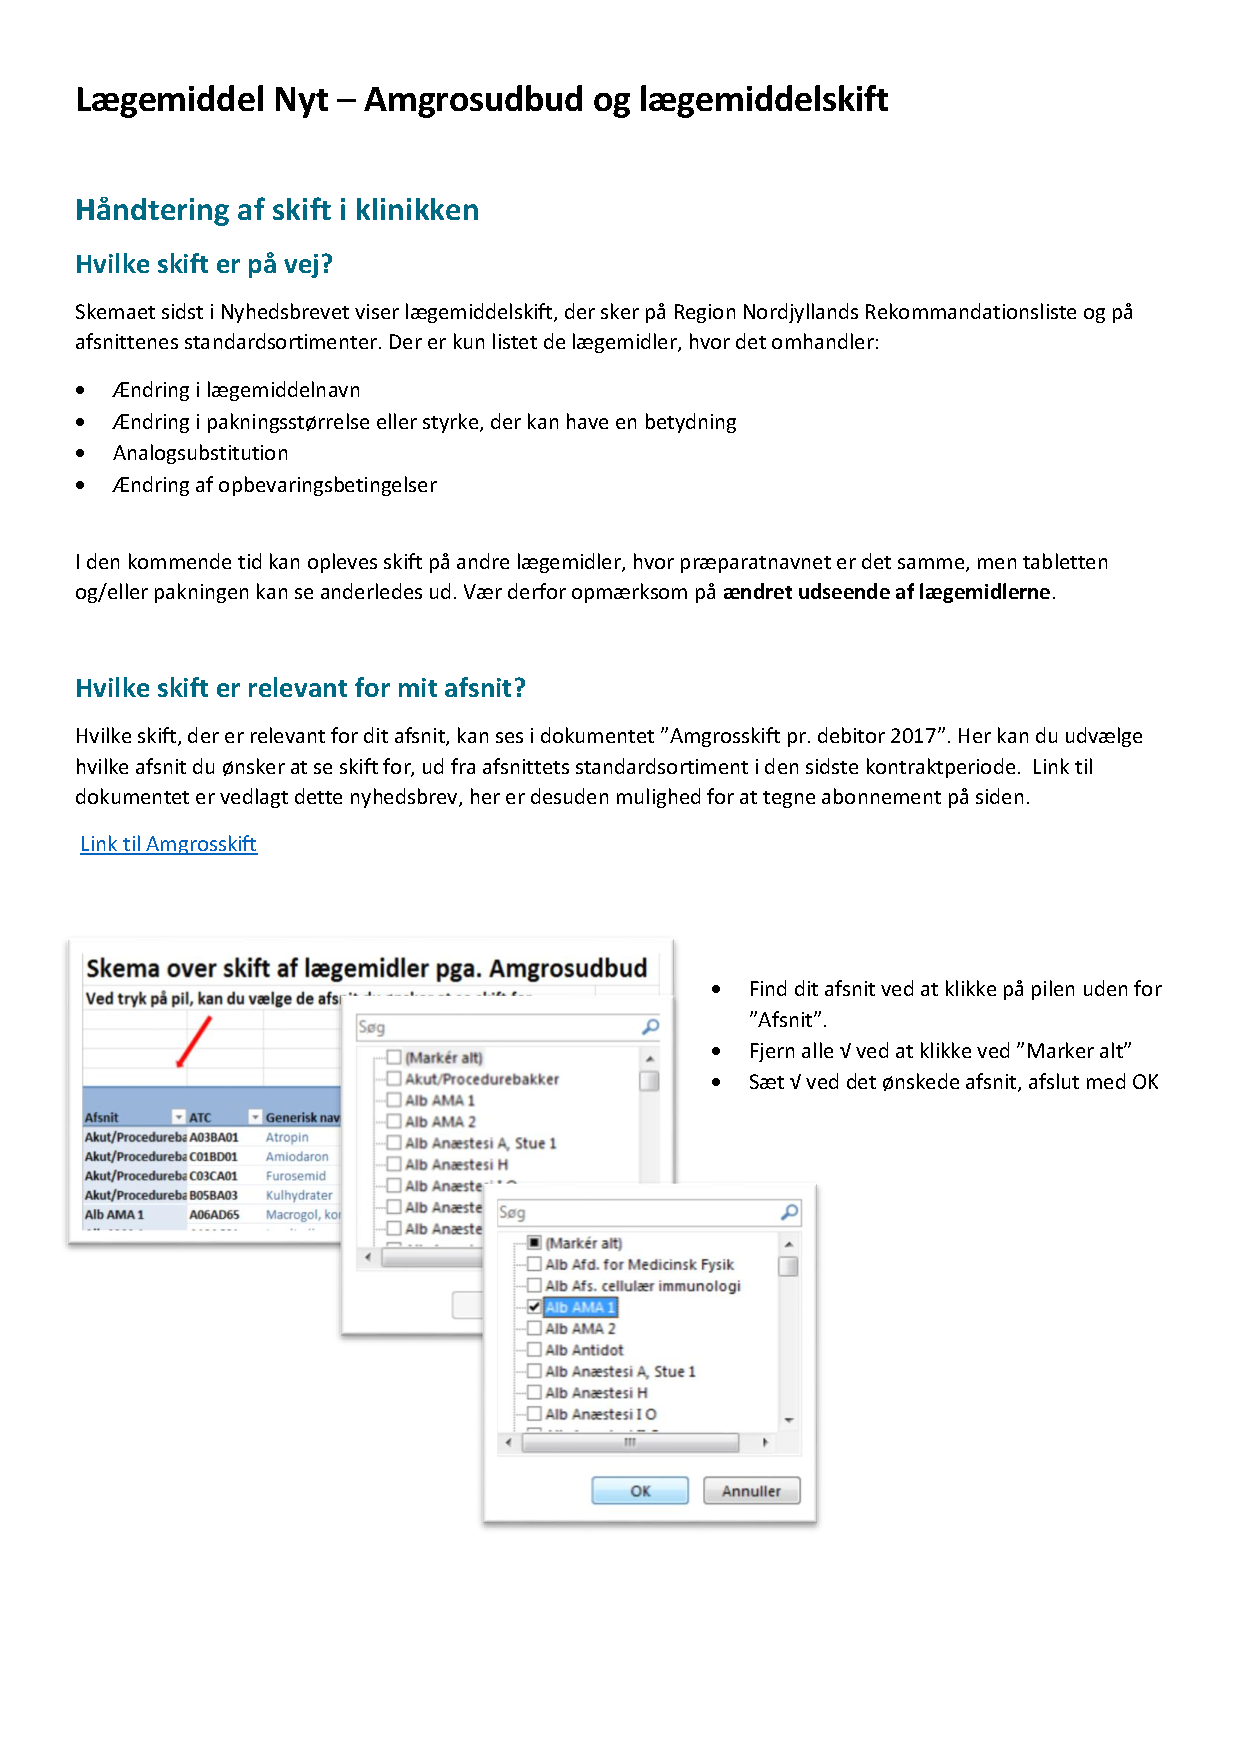
\includepdf[pages=1-10]{appendiks/Laegemiddelnyt.pdf}
														% Appendiks/bilag start - giver chapter bogstaver i stedet for tal
\clearforchapter												% Sikrer at pagestylen aktiveres paa den rigtige side
\phantomsection													% Kunstigt afsnit, som hyperlinks kan 'holde fast i'
\pdfbookmark[0]{Appendiks}{appendiks}							% Tildeler en klikbar bookmark til den endelige PDF

%% Indstillinger for appendiks (deaktiveret med "%") %%

%\pagestyle{empty}												% Sidehoved/-fod for standardsider aendres til tom for appendiks
%\aliaspagestyle{chapter}{empty}								% Sidehoved/-fod for kapitelsider aendres til tom for appendiks
%\settocdepth{chapter}											% Kun kapitel-niveau vises i ToC
%\addtocontents{toc}{\protect\cftpagenumbersoff{chapter}}		% Sidetal for kapitler fjernes i ToC

%% Filer til appendiks %%
%\include{appendiks/appendiks1}


%%%% Bilag %%%%

%\phantomsection												% Kunstigt afsnit, som hyperlinks kan 'holde fast i'
%\addcontentsline{toc}{chapter}{Bilag A \ Navn} 				% Manuelle indgange i indholdsfortegnelsen (naar \includepdf bruges)

%\includepdf[pages={x-y}]{filnavn}								% Inkluder eksterne bilag med \includepdf[pages={x-y}]{filnavn}


\end{document}													% Slutter dokumentet - obligatorisk


